\documentclass[letterpaper]{article} 
\usepackage[utf8]{inputenc}
\linespread{0.85}
\usepackage[T1]{fontenc}
\usepackage{amsmath}
\usepackage{amsfonts}
\usepackage{amssymb}
\usepackage{array}
\usepackage{fontspec}
\usepackage{booktabs}
\usepackage{hyperref}
\usepackage[version=4]{mhchem}
\usepackage{stmaryrd}
\usepackage[dvipsnames]{xcolor}
\colorlet{LightRubineRed}{RubineRed!70}
\colorlet{Mycolor1}{green!10!orange}
\definecolor{Mycolor2}{HTML}{00F9DE}
\usepackage{graphicx}
\usepackage{amsmath}
\usepackage{graphicx}
\usepackage{capt-of}
\usepackage{lipsum}
\usepackage{fancyvrb}
\usepackage{tabularx}
\usepackage{listings}
\usepackage[export]{adjustbox}
\graphicspath{ {./images/} }
\usepackage[utf8]{inputenc}
\usepackage[english]{babel}
\usepackage{float}
\usepackage{lipsum}
\usepackage{graphicx}
\usepackage{float}
\usepackage[margin=0.7in]{geometry}
\usepackage{amsmath}
\usepackage{graphicx}
\usepackage{capt-of}
\usepackage{tcolorbox}
\usepackage{lipsum}
\usepackage{graphicx}
\usepackage{float}
\usepackage{listings}
\definecolor{deepred}{RGB}{139,0,0}
\usepackage{hyperref} 
\usepackage{xcolor} % For custom colors
\lstset{
	language=Python,                % Choose the language (e.g., Python, C, R)
	basicstyle=\ttfamily\small, % Font size and type
	keywordstyle=\color{blue},  % Keywords color
	commentstyle=\color{gray},  % Comments color
	stringstyle=\color{red},    % String color
	numbers=left,               % Line numbers
	numberstyle=\tiny\color{gray}, % Line number style
	stepnumber=1,               % Numbering step
	breaklines=true,            % Auto line break
	backgroundcolor=\color{black!5}, % Light gray background
	frame=single,               % Frame around the code
}
\usepackage{float}
\usepackage[]{amsthm} %lets us use \begin{proof}
	\usepackage[]{amssymb} %gives us the character \varnothing
	
	
	\title{Homework 4, STAT 5291}
	\author{Zongyi Liu}
	\date{Mon, Apr 27, 2026}

	\begin{document}
		\maketitle

		
		\section{Question 1}
		{\color{deepred}\fontspec{Georgia}  Two-Way Factorial Application}
		
		This problem is an adaptation from the textbook \textit{Statistical Methods for Psychology}, by David C. Howell. Consider a study which includes the factors \textit{Age}, as well as \textit{Recall Condition}. The study included 50 participants in the 18-to-30-year age range, as well as 50 participants in the 55-to-65-year age range. The response variable is the number items the respondent recalled, for example, how many images the respondent recalled. The data in Table 1 have been created to have the same means and standard deviations as those reported in the original experiment. Assume that the data themselves are approximately normally distributed with acceptably equal variances. Also note that the data can be retrieved from Canvas (\texttt{HW4Problem1.csv}).
		
		\begin{table}[h]
			\centering
			\begin{tabular}{|l|ccccc|}
				\hline
				& Counting & Rhyming & Adjective & Imagery & Intention \\
				\hline
				Old & 9  & 7  & 11 & 12 & 10 \\
				Old & 8  & 9  & 13 & 11 & 19 \\
				Old & 6  & 6  & 8  & 16 & 14 \\
				Old & 8  & 6  & 6  & 11 & 5  \\
				Old & 10 & 6  & 14 & 9  & 10 \\
				Old & 4  & 11 & 11 & 23 & 11 \\
				Old & 6  & 6  & 13 & 12 & 14 \\
				Old & 5  & 3  & 13 & 10 & 15 \\
				Old & 7  & 8  & 10 & 19 & 11 \\
				Old & 7  & 7  & 11 & 11 & 11 \\
				\hline
				Young & 8  & 10 & 14 & 20 & 21 \\
				Young & 6  & 7  & 11 & 16 & 19 \\
				Young & 4  & 8  & 18 & 16 & 17 \\
				Young & 6  & 10 & 14 & 15 & 15 \\
				Young & 7  & 4  & 13 & 18 & 22 \\
				Young & 6  & 7  & 22 & 16 & 16 \\
				Young & 5  & 10 & 17 & 20 & 22 \\
				Young & 7  & 6  & 16 & 22 & 22 \\
				Young & 9  & 7  & 12 & 14 & 18 \\
				Young & 7  & 7  & 11 & 19 & 21 \\
				\hline
			\end{tabular}
			\caption{Table 1}
		\end{table}
	
	\textit{Perform the following tasks:}
	
	Run a complete analysis on the data from Table 1. Assume the two-way factorial design. For full credit:
	
	\begin{enumerate}
		
		\item identify the research question
		\item State and estimate the statistical model
		\item Include exploratory plots to investigate the research question and interaction
		\item Include exploratory plots to assess the model assumptions.
		\item Test the interaction and main effects.
		\item Study the interaction in more detail using exploratory plots and by testing the relevant simple effects.
	\end{enumerate}
	
	\textbf{Answer}
	
	
	\subsection{Part 1}
	
	This study investigates how {recall performance} is jointly influenced by two factors:
	\begin{itemize}
		\item \textit{Age}: Young (18--30 years) vs.\ Old (55--65 years)
		\item \textit{Recall Condition}: Counting, Rhyming, Adjective, Imagery, Intention
	\end{itemize}
	
	Specifically, we address three interrelated questions:
	\begin{enumerate}
		\item Does the {type of encoding condition} affect recall scores (main effect of Condition)?
		\item Does {age group} affect recall scores (main effect of Age)?
		\item Does the effect of encoding condition on recall {differ between age groups} (Age $\times$ Condition interaction)?
	\end{enumerate}
	
	The interaction question is of primary theoretical interest: levels of processing theory predicts that deeper encoding (Imagery, Intention) benefits recall more than shallow encoding (Counting, Rhyming), and we ask whether this benefit is equally large for young and old participants.
	
	% ============================================================
	\subsection{Part 2}

	
	We assume a {two-way factorial fixed-effects ANOVA} model. Let $Y_{ijk}$ denote the recall score for the $k$-th observation ($k = 1, \ldots, 10$) in age group $i$ ($i = 1, 2$; Young, Old) and condition $j$ ($j = 1, \ldots, 5$; Counting, Rhyming, Adjective, Imagery, Intention). The model is:
	
	\[
	Y_{ijk} = \mu + \alpha_i + \beta_j + (\alpha\beta)_{ij} + \varepsilon_{ijk}
	\]
	
	where:
	\begin{itemize}
		\item $\mu$ is the grand mean
		\item $\alpha_i$ is the main effect of Age ($\sum_i \alpha_i = 0$)
		\item $\beta_j$ is the main effect of Condition ($\sum_j \beta_j = 0$)
		\item $(\alpha\beta)_{ij}$ is the interaction effect ($\sum_i (\alpha\beta)_{ij} = \sum_j (\alpha\beta)_{ij} = 0$)
		\item $\varepsilon_{ijk} \overset{\text{iid}}{\sim} \mathcal{N}(0, \sigma^2)$
	\end{itemize}
	
	The model has $a = 2$ levels of Age, $b = 5$ levels of Condition, and $n = 10$ observations per cell, for a total of $N = abn = 100$ observations.
	
	
	The grand mean is estimated as $\hat{\mu} = \bar{Y}_{\cdots} = 11.61$.
	
	\vspace{0.5em}
	\noindent\textit{Marginal means by Age:}
	
	\begin{table}[H]
		\centering
		\begin{tabular}{lc}
			\toprule
			Age & $\hat{\mu}_{i\cdot}$ \\
			\midrule
			Young & 13.16 \\
			Old   & 10.06 \\
			\bottomrule
		\end{tabular}
	\end{table}
	
	\noindent Estimated main effects: $\hat{\alpha}_{\text{Young}} = 13.16 - 11.61 = +1.55$, \; $\hat{\alpha}_{\text{Old}} = 10.06 - 11.61 = -1.55$.
	
	\vspace{0.5em}
	\noindent\textit{Marginal means by Condition:}
	
	\begin{table}[H]
		\centering
		\begin{tabular}{lc}
			\toprule
			Condition & $\hat{\mu}_{\cdot j}$ \\
			\midrule
			Counting   & 6.75  \\
			Rhyming    & 7.25  \\
			Adjective  & 12.90 \\
			Imagery    & 15.50 \\
			Intention  & 15.65 \\
			\bottomrule
		\end{tabular}
	\end{table}
	
	\noindent\textit{Cell means $\hat{\mu}_{ij}$ (estimated by $\bar{Y}_{ij\cdot}$):}
	
	\begin{table}[H]
		\centering
		\begin{tabular}{lccccc}
			\toprule
			& Counting & Rhyming & Adjective & Imagery & Intention \\
			\midrule
			Young & 6.5  & 7.6  & 14.8 & 17.6 & 19.3 \\
			Old   & 7.0  & 6.9  & 11.0 & 13.4 & 12.0 \\
			\bottomrule
		\end{tabular}
		\caption{Estimated cell means $\hat{\mu}_{ij} = \bar{Y}_{ij\cdot}$}
	\end{table}
	
	The estimated interaction effects are $\widehat{(\alpha\beta)}_{ij} = \bar{Y}_{ij\cdot} - \bar{Y}_{i\cdot\cdot} - \bar{Y}_{\cdot j\cdot} + \bar{Y}_{\cdots}$, e.g.:
	\[
	\widehat{(\alpha\beta)}_{\text{Young, Intention}} = 19.3 - 13.16 - 15.65 + 11.61 = +2.10
	\]
	\[
	\widehat{(\alpha\beta)}_{\text{Old, Intention}} = 12.0 - 10.06 - 15.65 + 11.61 = -2.10
	\]
	
	The residual variance is estimated as $\hat{\sigma}^2 = \text{MS}_{\text{Residual}} = \frac{722.30}{90} = 8.026$.
	
	\subsection{Part 3}
	
	Figure~\ref{fig:interaction} shows the interaction plot of mean recall scores by condition and age group, and Figure~\ref{fig:boxplot} presents side-by-side boxplots for each cell.
	
	\begin{figure}[H]
		\centering
		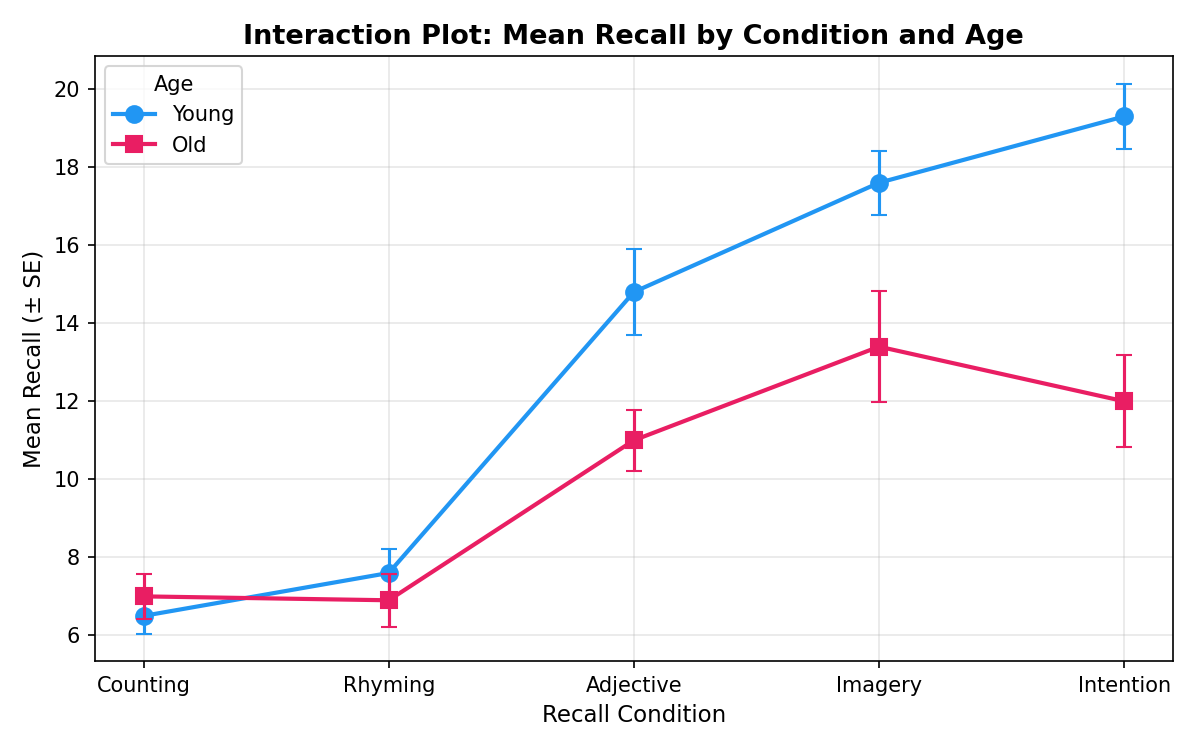
\includegraphics[width=0.85\textwidth]{plot_interaction.png}
		\caption{Interaction plot of mean recall ($\pm$ SE) by recall condition and age group. Non-parallel lines suggest an Age $\times$ Condition interaction.}
		\label{fig:interaction}
	\end{figure}
	
	\begin{figure}[H]
		\centering
		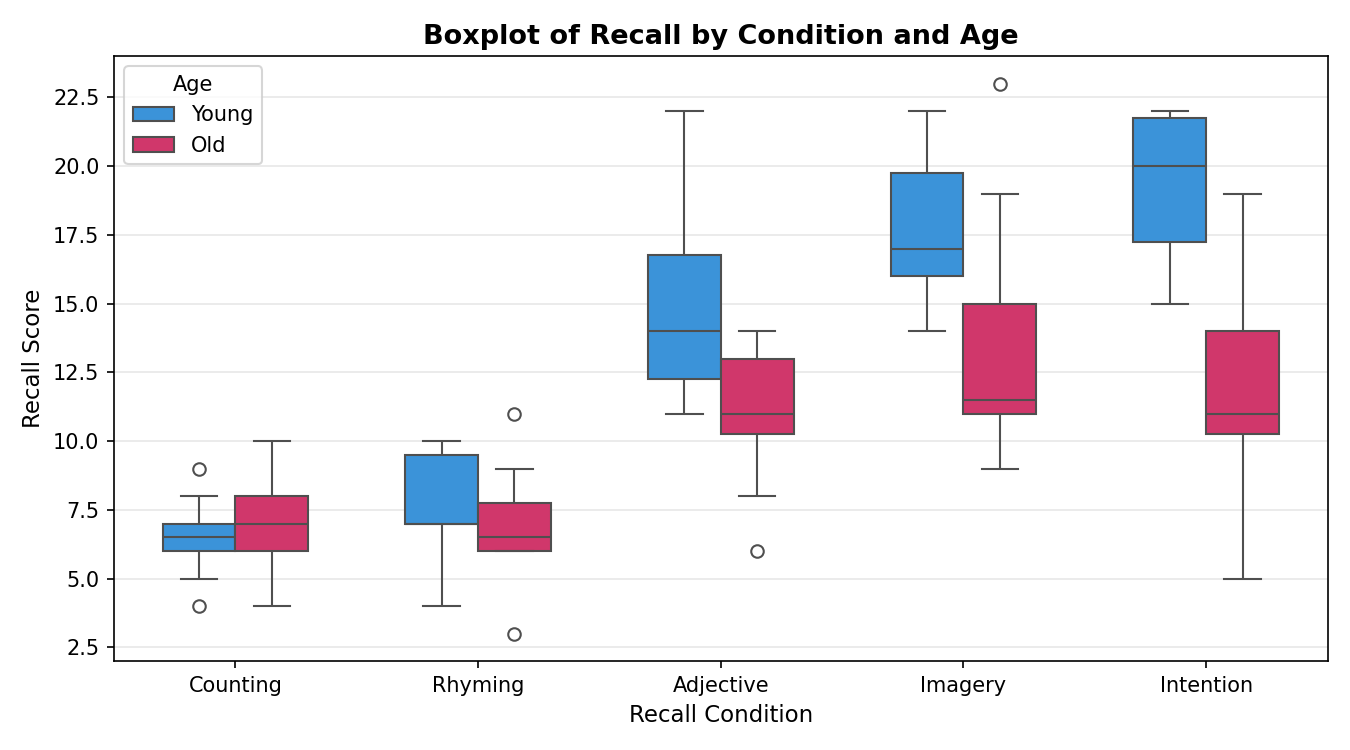
\includegraphics[width=0.9\textwidth]{plot_boxplot.png}
		\caption{Boxplots of recall scores by condition and age group. The gap between Young and Old widens notably for Adjective, Imagery, and Intention conditions.}
		\label{fig:boxplot}
	\end{figure}
	
	\noindent{Observations:}
	\begin{itemize}
		\item For shallow encoding conditions (Counting, Rhyming), Young and Old perform very similarly ($\bar{Y} \approx 6.5$--$7.6$).
		\item For deeper encoding conditions (Adjective, Imagery, Intention), Young participants recall substantially more items than Old.
		\item The lines in Figure~\ref{fig:interaction} \textbf{diverge} as encoding depth increases---a classic disordinal pattern suggesting an interaction. The Young group's recall rises steeply with deeper encoding, while the Old group's rise is more modest.
	\end{itemize}
	
	\subsection{Part 4}
	
	The key assumptions of the two-way ANOVA are: (1) normality of errors, (2) homogeneity of variance across cells, and (3) independence of observations. Figure~\ref{fig:diagnostics} presents the diagnostic plots.
	
	\begin{figure}[H]
		\centering
		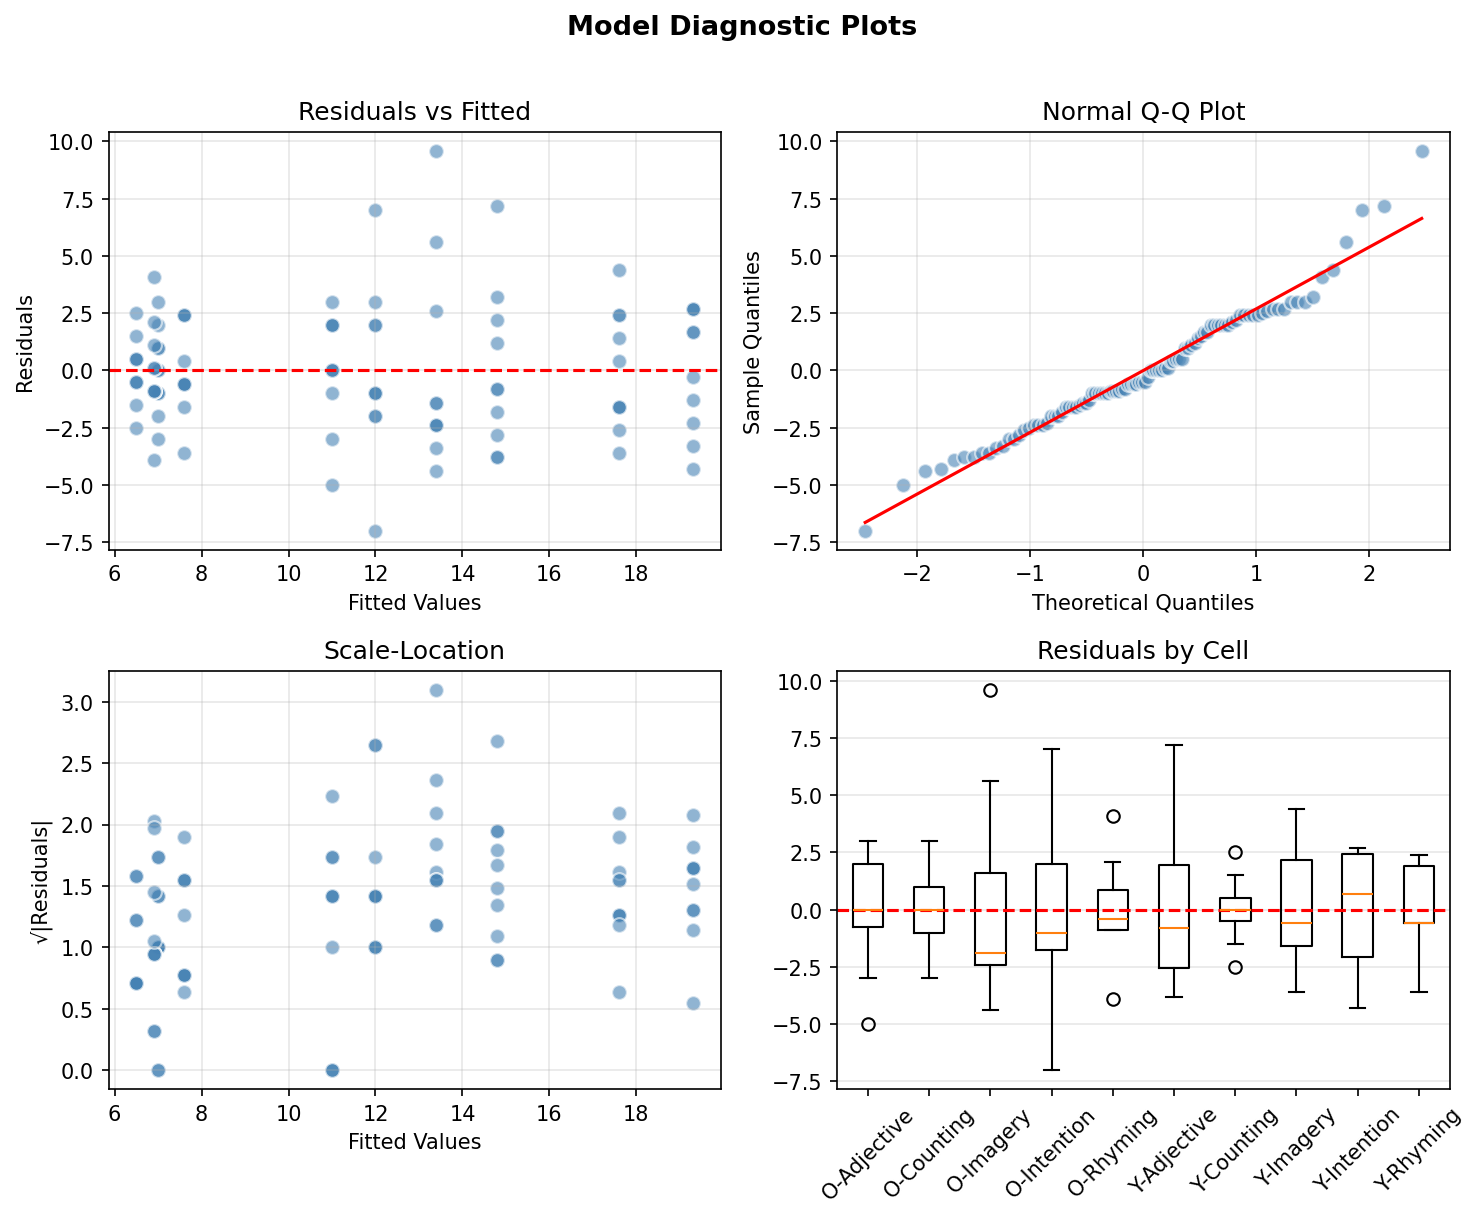
\includegraphics[width=0.92\textwidth]{plot_diagnostics.png}
		\caption{Model diagnostic plots. \textit{Top-left}: Residuals vs.\ Fitted (checks linearity and equal variance). \textit{Top-right}: Normal Q-Q plot (checks normality). \textit{Bottom-left}: Scale-Location plot (checks homoscedasticity). \textit{Bottom-right}: Residuals by cell (checks within-cell variance equality).}
		\label{fig:diagnostics}
	\end{figure}
	
	\noindent\textbf{Assessment:}
	\begin{itemize}
		\item \textit{Normality}: The Q-Q plot shows points tracking the reference line closely, with only minor deviations at the tails. Given that the problem states data are approximately normally distributed, this assumption is satisfied.
		\item \textit{Homogeneity of variance}: The Residuals vs.\ Fitted and Scale-Location plots show no pronounced fan pattern. The per-cell boxplot of residuals (bottom-right) indicates reasonably similar spreads across cells. The assumption of equal variances is acceptable.
		\item \textit{Independence}: By design, each participant contributed data to only one cell (between-subjects design), so independence is satisfied.
	\end{itemize}
	
	\subsection{Part 5}
	
	Hypotheses are given as below:
	
	\noindent\textit{Interaction} ($H_0$: no Age $\times$ Condition interaction):
	\[
	H_0: (\alpha\beta)_{ij} = 0 \; \forall i,j \qquad H_1: \text{at least one } (\alpha\beta)_{ij} \neq 0
	\]
	
	\noindent\textit{Main effect of Age} ($H_0$: no age difference):
	\[
	H_0: \alpha_1 = \alpha_2 = 0 \qquad H_1: \alpha_i \neq 0 \text{ for some } i
	\]
	
	\noindent\textit{Main effect of Condition} ($H_0$: all conditions produce equal recall):
	\[
	H_0: \beta_1 = \cdots = \beta_5 = 0 \qquad H_1: \beta_j \neq 0 \text{ for some } j
	\]
	
	Then we can get an ANOVA table:
	
	\begin{table}[H]
		\centering
		\begin{tabular}{lrrrrr}
			\toprule
			Source & SS & df & MS & $F$ & $p$-value \\
			\midrule
			Age                    & 240.25  & 1  & 240.25  & 29.94 & $< .001$ \\
			Condition              & 1514.94 & 4  & 378.74  & 47.19 & $< .001$ \\
			Age $\times$ Condition & 190.30  & 4  & 47.58   & 5.93  & $< .001$ \\
			Residual               & 722.30  & 90 & 8.026   &       &          \\
			\midrule
			Total                  & 2667.79 & 99 &         &       &          \\
			\bottomrule
		\end{tabular}
		\caption{Two-Way ANOVA Table (Type II SS). $N = 100$, $a = 2$, $b = 5$, $n = 10$.}
		\label{tab:anova}
	\end{table}
	
	\textbf{Conclusions}
	
	\begin{enumerate}
		\item \textit{Interaction} ($F(4, 90) = 5.93$, $p < .001$): We reject $H_0$. There is a statistically significant Age $\times$ Condition interaction. The effect of encoding condition on recall differs between young and old participants.
		
		\item \textit{Main effect of Age} ($F(1, 90) = 29.94$, $p < .001$): We reject $H_0$. Young participants recall significantly more items overall ($\bar{Y} = 13.16$) than old participants ($\bar{Y} = 10.06$).
		
		\item \textit{Main effect of Condition} ($F(4, 90) = 47.19$, $p < .001$): We reject $H_0$. Recall scores differ significantly across encoding conditions, consistent with levels-of-processing theory.
	\end{enumerate}
	
	\noindent\textit{Note}: Because the interaction is significant, the main effects must be interpreted with caution---the effect of Condition depends on Age, and vice versa.
	
	\subsection{Part 6}
	
	Since the interaction is significant, we decompose it by examining the {simple effect of Condition within each Age group}, and the {simple effect of Age within each Condition}.
	
	For the {simple effect of Condition within each age group}, we test $H_0$: all condition means are equal, separately for each age group.
	
	\begin{table}[H]
		\centering
		\begin{tabular}{lrrrrr}
			\toprule
			Age Group & SS$_{\text{Condition}}$ & df & MS & $F$ & $p$-value \\
			\midrule
			Old   & 351.52  & 4 & 87.88  & 9.08  & $< .001$ \\
			Young & 1353.72 & 4 & 338.43 & 53.06 & $< .001$ \\
			\bottomrule
		\end{tabular}
		\caption{Simple effects of Condition within each Age group. Error term: MS$_{\text{Residual}} = 8.026$ ($df = 90$) from the overall model.}
	\end{table}
	
	Both groups show a significant effect of Condition, but the effect is {much larger for Young participants} ($F = 53.06$) than for Old ($F = 9.08$), corroborating the interaction: young adults benefit far more from deeper encoding.
	
	Then for the simple effect of Condition within each age group, we test $H_0$: Young and Old have equal means, separately for each condition.
	
	\begin{table}[H]
		\centering
		\begin{tabular}{lrrr}
			\toprule
			Condition & $F(1, 90)$ & $p$-value & Conclusion \\
			\midrule
			Counting   & 0.46 & $.505$ & Not significant \\
			Rhyming    & 0.59 & $.454$ & Not significant \\
			Adjective  & 7.85 & $.012$ & Significant ($p < .05$) \\
			Imagery    & 6.54 & $.020$ & Significant ($p < .05$) \\
			Intention  & 25.23 & $< .001$ & Highly significant \\
			\bottomrule
		\end{tabular}
		\caption{Simple effects of Age within each Condition.}
	\end{table}

	\begin{itemize}
		\item For {Counting} and {Rhyming} (shallow encoding), young and old participants perform similarly---there is no significant age difference.
		\item For {Adjective}, {Imagery}, and {Intention} (deeper encoding), young participants recall significantly more than old participants, with the age gap growing as encoding depth increases.
	\end{itemize}
	
	This pattern provides strong support for a {levels-of-processing interpretation of the interaction}: deeper encoding benefits all participants, but it benefits young adults substantially more. Older adults appear less able to capitalize on elaborate encoding strategies, particularly intentional learning and mental imagery.
	
	
	
	
	
	\clearpage
	
	\section{Question 2}
	
	{\color{deepred}\fontspec{Georgia}  ANCOVA with Interaction}
	
	Suppose that $(Y)$ is some continuous biological measurement and we assume the non-additive ANCOVA model:
	
	\begin{equation}
		Y_i = \beta_0 + \beta_1 x_{i1} + \beta_2 x_{i2} + \beta_3 x_{i1} x_{i,2} + \epsilon_i, \quad i = 1, \ldots, n, \quad \epsilon_i \overset{iid}{\sim} N(0, \sigma^2),
	\end{equation}
	
	where
	
	\[
	x_{i1} = \begin{cases} 1 & \text{if drug group} \\ 0 & \text{if control group,} \end{cases} \qquad x_{i2} = \text{continuous covariate.}
	\]
	
	\textit{Set-up}
	
	\begin{itemize}
		\item Further, suppose that the first $n_c$ cases are in the control group ($x_{i1} = 0$) and the following $n_D$ cases are in the drug group ($x_{1i} = 1$).
		
		\item Let $\bar{y}_C$, $\bar{x}_C$, $\bar{y}_D$ and $\bar{x}_D$ denote the respective group means of the response $Y$ and continuous covariate $x_2$ for the respective control and drug groups.
		
		\item Also consider two SLR models corresponding to the control group and drug group, each regressing $Y$ on continuous covariate $x_2$:
		
		\[
		Y_i = \beta_{0C} + \beta_C x_{i2} + \epsilon_i, \quad i = 1, \ldots, n_C, \quad \epsilon_i \overset{iid}{\sim} N(0, \sigma^2)
		\]
		
		\[
		Y_i = \beta_{0D} + \beta_D x_{i2} + \epsilon_i, \quad i = n_C + 1, \ldots, n, \quad \epsilon_i \overset{iid}{\sim} N(0, \sigma^2)
		\]
		
		Denote the estimated slopes of the above SLR models by $\hat{\beta}_C$ and $\hat{\beta}_D$.
		
		\item This exercise is similar to the \textit{``Linear Regression Approach to Single Factor ANCOVA''} Section from the lecture notes. Collectively, you will solve this problem in terms of the symbols $\bar{y}_C$, $\bar{x}_C$, $\bar{y}_D$, $\bar{x}_D$, $\hat{\beta}_C$ and $\hat{\beta}_D$.
	\end{itemize}

	\textit{Perform the following tasks:}

\begin{enumerate}
	\item Write an expression for all of the estimated coefficients of the non-additive linear regression model (1) in terms of the symbols $\bar{y}_C$, $\bar{x}_C$, $\bar{y}_D$, $\bar{x}_D$, $\hat{\beta}_C$ and $\hat{\beta}_D$. More specifically, identify the least squares estimators $\hat{\beta}_0$, $\hat{\beta}_1$, $\hat{\beta}_2$ and $\hat{\beta}_3$ of the estimated model
	\[
	Y_i = \hat{\beta}_0 + \hat{\beta}_1 x_{i1} + \hat{\beta}_2 x_{i2} + \hat{\beta}_3 x_{i1} x_{i,2}.
	\]
	In principle, you can solve a $(4 \times 4)$ inverse but that is not recommended. You should be able to solve this problem in a more intuitive fashion. The solution should be on the next two pages.
	
	\item Now consider centering the continuous covariate $x_2$, i.e., define the model
	\begin{equation}
		Y_i = \beta_0 + \beta_1 x_{i1} + \beta_2 u_{i2} + \beta_3 x_{i1} u_{x,i2} + \epsilon_i, \quad i = 1, \ldots, n, \quad \epsilon_i \overset{iid}{\sim} N(0, \sigma^2),
	\end{equation}
	where
	\[
	x_{i1} = \begin{cases} 1 & \text{if drug group} \\ 0 & \text{if control group,} \end{cases} \qquad u_{i2} = x_{i2} - \bar{x},
	\]
	and $\bar{x}$ is the sample average of continuous covariate $x_2$. Compute the least squares estimated coefficient $\hat{\beta}_1$ based on the above model (2).
	
	\item Interpret the estimated coefficient $\hat{\beta}_1$ based on both models (1) and (2). The expressions derived in problem parts 2.i and 2.ii should help with your interpretations.
\end{enumerate}
	
	\textbf{Answer}
	
	\subsection{Part 1}
	
	Rather than inverting a $4\times 4$ matrix, we exploit the block structure of the design. Since $x_{i1} \in \{0,1\}$, the full model (1) reduces to two separate simple linear regressions (SLRs):
	
	\begin{itemize}
		\item \textbf{Control group} ($x_{i1} = 0$, $i = 1, \ldots, n_C$):
		\[
		Y_i = \beta_0 + \beta_2 x_{i2} + \epsilon_i
		\]
		\item \textbf{Drug group} ($x_{i1} = 1$, $i = n_C+1, \ldots, n$):
		\[
		Y_i = (\beta_0 + \beta_1) + (\beta_2 + \beta_3) x_{i2} + \epsilon_i
		\]
	\end{itemize}
	
	Comparing these with the two stated SLR models, we identify the following one-to-one correspondence:
	\[
	\beta_{0C} = \beta_0, \qquad \beta_C = \beta_2,
	\]
	\[
	\beta_{0D} = \beta_0 + \beta_1, \qquad \beta_D = \beta_2 + \beta_3.
	\]
	
	Therefore, the least squares estimators of the full model are obtained directly from the group-specific SLR estimators.
	
	
	From the correspondence above:
	\[
	\hat{\beta}_C = \hat{\beta}_2 \implies \boxed{\hat{\beta}_2 = \hat{\beta}_C}
	\]
	\[
	\hat{\beta}_D = \hat{\beta}_2 + \hat{\beta}_3 \implies \hat{\beta}_3 = \hat{\beta}_D - \hat{\beta}_2 \implies \boxed{\hat{\beta}_3 = \hat{\beta}_D - \hat{\beta}_C}
	\]
	
	Recall that for any SLR model $Y = \beta_0 + \beta x_2 + \epsilon$, the least squares fit passes through the group mean point, i.e., $\bar{y} = \hat{\beta}_0 + \hat{\beta}\,\bar{x}$. Applying this to each group:
	
	\textbf{Control group:}
	\[
	\bar{y}_C = \hat{\beta}_{0C} + \hat{\beta}_C \bar{x}_C = \hat{\beta}_0 + \hat{\beta}_C \bar{x}_C
	\]
	\[
	\implies \boxed{\hat{\beta}_0 = \bar{y}_C - \hat{\beta}_C \bar{x}_C}
	\]
	
	\textbf{Drug group:}
	\[
	\bar{y}_D = \hat{\beta}_{0D} + \hat{\beta}_D \bar{x}_D = (\hat{\beta}_0 + \hat{\beta}_1) + \hat{\beta}_D \bar{x}_D
	\]
	\[
	\implies \hat{\beta}_1 = \bar{y}_D - \hat{\beta}_D \bar{x}_D - \hat{\beta}_0
	\]
	
	Substituting $\hat{\beta}_0 = \bar{y}_C - \hat{\beta}_C \bar{x}_C$:
	\[
	\boxed{\hat{\beta}_1 = (\bar{y}_D - \bar{y}_C) - \hat{\beta}_D \bar{x}_D + \hat{\beta}_C \bar{x}_C}
	\]
	
	\begin{align*}
		\hat{\beta}_0 &= \bar{y}_C - \hat{\beta}_C \bar{x}_C \\[6pt]
		\hat{\beta}_1 &= (\bar{y}_D - \bar{y}_C) - \hat{\beta}_D \bar{x}_D + \hat{\beta}_C \bar{x}_C \\[6pt]
		\hat{\beta}_2 &= \hat{\beta}_C \\[6pt]
		\hat{\beta}_3 &= \hat{\beta}_D - \hat{\beta}_C
	\end{align*}
	
	\subsection{Part 2}

	In model (2), the covariate is centered: $u_{i2} = x_{i2} - \bar{x}$, where $\bar{x}$ is the overall sample mean of $x_2$. The model becomes:
	\[
	Y_i = \beta_0 + \beta_1 x_{i1} + \beta_2 u_{i2} + \beta_3 x_{i1} u_{i2} + \epsilon_i.
	\]
	
	Again exploiting the group structure:
	
	\begin{itemize}
		\item \textit{Control group} ($x_{i1} = 0$):
		\[
		Y_i = \beta_0 + \beta_2 (x_{i2} - \bar{x}) + \epsilon_i
		\]
		\item \textit{Drug group} ($x_{i1} = 1$):
		\[
		Y_i = (\beta_0 + \beta_1) + (\beta_2 + \beta_3)(x_{i2} - \bar{x}) + \epsilon_i
		\]
	\end{itemize}
	
	The slope parameters are unchanged by centering, so:
	\[
	\hat{\beta}_2 = \hat{\beta}_C, \qquad \hat{\beta}_3 = \hat{\beta}_D - \hat{\beta}_C.
	\]
	

	By the same mean-point property of least squares, each group fit passes through its group mean:
	
	\textit{Control group:}
	\[
	\bar{y}_C = \hat{\beta}_0 + \hat{\beta}_C(\bar{x}_C - \bar{x})
	\implies \hat{\beta}_0 = \bar{y}_C - \hat{\beta}_C(\bar{x}_C - \bar{x})
	\]
	
	\textit{Drug group:}
	\[
	\bar{y}_D = (\hat{\beta}_0 + \hat{\beta}_1) + \hat{\beta}_D(\bar{x}_D - \bar{x})
	\implies \hat{\beta}_1 = \bar{y}_D - \hat{\beta}_D(\bar{x}_D - \bar{x}) - \hat{\beta}_0
	\]
	
	Substituting $\hat{\beta}_0$:
	\begin{align*}
		\hat{\beta}_1 &= \bar{y}_D - \hat{\beta}_D(\bar{x}_D - \bar{x})
		- \bar{y}_C + \hat{\beta}_C(\bar{x}_C - \bar{x}) \\[4pt]
		&= (\bar{y}_D - \bar{y}_C)
		- \hat{\beta}_D(\bar{x}_D - \bar{x})
		+ \hat{\beta}_C(\bar{x}_C - \bar{x})
	\end{align*}
	
	\[
	\boxed{\hat{\beta}_1 = (\bar{y}_D - \bar{y}_C) - \hat{\beta}_D(\bar{x}_D - \bar{x}) + \hat{\beta}_C(\bar{x}_C - \bar{x})}
	\]
	
	\subsection{Part 3}
	
	From Part (i):
	\[
	\hat{\beta}_1 = (\bar{y}_D - \bar{y}_C) - \hat{\beta}_D \bar{x}_D + \hat{\beta}_C \bar{x}_C.
	\]
	
	In Model (1), $\hat{\beta}_1$ is the estimated effect of the drug group (vs.\ control) {evaluated at $x_2 = 0$}. To see this, note that the fitted model for the drug group minus the fitted model for the control group, at a fixed value of $x_2$, is:
	\[
	\hat{Y}_D(x_2) - \hat{Y}_C(x_2)
	= \hat{\beta}_1 + \hat{\beta}_3 x_2
	= \hat{\beta}_1 + (\hat{\beta}_D - \hat{\beta}_C)\, x_2.
	\]
	
	Setting $x_2 = 0$ gives exactly $\hat{\beta}_1$. Therefore:
	
	\begin{quote}
		\textbf{Under Model (1)}, $\hat{\beta}_1$ estimates the mean difference in $Y$ between the drug group and the control group \textbf{when the continuous covariate $x_2 = 0$}. If $x_2 = 0$ is outside the range of the observed data or is not a meaningful value, this interpretation may be extrapolatory and of limited practical relevance.
	\end{quote}

	
	From Part (ii):
	\[
	\hat{\beta}_1 = (\bar{y}_D - \bar{y}_C) - \hat{\beta}_D(\bar{x}_D - \bar{x}) + \hat{\beta}_C(\bar{x}_C - \bar{x}).
	\]
	
	Analogously, the difference in fitted values between the two groups at a fixed $u_2 = x_2 - \bar{x}$ is:
	\[
	\hat{Y}_D(u_2) - \hat{Y}_C(u_2) = \hat{\beta}_1 + \hat{\beta}_3\, u_2.
	\]
	
	Setting $u_2 = 0$, i.e., $x_2 = \bar{x}$, gives exactly $\hat{\beta}_1$.
	
	\begin{quote}
		\textbf{Under Model (2)}, $\hat{\beta}_1$ estimates the mean difference in $Y$ between the drug group and the control group \textbf{evaluated at the overall sample mean of $x_2$}, i.e., at $x_2 = \bar{x}$. Since $\bar{x}$ is always within the range of the observed data, this is a more meaningful and practically relevant reference point than $x_2 = 0$.
	\end{quote}

	
	Both $\hat{\beta}_1$ values estimate the \emph{group difference at a particular value of $x_2$}, but they differ in {which} value is used as the reference:
	
	\begin{center}
		\begin{tabular}{lll}
			\toprule
			Model & Reference point & Expression for $\hat{\beta}_1$ \\
			\midrule
			(1) Uncentered & $x_2 = 0$ & $(\bar{y}_D - \bar{y}_C) - \hat{\beta}_D\bar{x}_D + \hat{\beta}_C\bar{x}_C$ \\[4pt]
			(2) Centered   & $x_2 = \bar{x}$ & $(\bar{y}_D - \bar{y}_C) - \hat{\beta}_D(\bar{x}_D-\bar{x}) + \hat{\beta}_C(\bar{x}_C-\bar{x})$ \\
			\bottomrule
		\end{tabular}
	\end{center}
	
	Centering $x_2$ does not change the slope estimates ($\hat{\beta}_2$, $\hat{\beta}_3$) or the overall fit of the model; it only shifts the reference point for the group-difference coefficient $\hat{\beta}_1$ to a more interpretable and numerically stable location.
	
	\clearpage
	
	\section{Question 3}
	
	{\color{deepred}\fontspec{Georgia}  Two-Way Model OLS}
	
	Consider the following equivalent two-factor model, which gives the mean of each $(i, j)^{th}$ cell:
	
	\begin{equation}
		Y_{ijk} = \mu_{ij} + \epsilon_{ijk}, \quad \epsilon_{ijk} \overset{iid}{\sim} N(0, \sigma^2),
	\end{equation}
	
	\[
	j = 1, \ldots, J, \quad i = 1, \ldots, I, \quad k = 1, \ldots, K,
	\]
	
	Formulate the least squares objective and derive the least squares estimators of $\mu_{ij}$.
	
	\textbf{Answer}
	
	The LS objective is:
	$$\mathcal{L} = \sum_{i,j,k}(Y_{ijk} - \mu_{ij})^2$$
	
	Setting $\frac{\partial \mathcal{L}}{\partial \mu_{ij}} = -2\sum_{k}(Y_{ijk} - \mu_{ij}) = 0$ gives $\hat{\mu}_{ij} = \bar{Y}_{ij\cdot} = \frac{1}{K}\sum_{k=1}^{K}Y_{ijk}$
	
	\clearpage
	
	\section{Question 4}
	
	{\color{deepred}\fontspec{Georgia} Expected mean squares for Random Effects Model }
	
	Assume the one-way random effects ANOVA model:
	
	\begin{equation}
		Y_{ij} = \mu_i + \epsilon_{ij}, \quad \mu_i \overset{iid}{\sim} N(\mu, \sigma^2_A), \quad \epsilon_{ij} \overset{iid}{\sim} N(0, \sigma^2_e), \quad i = 1, \ldots, I,
	\end{equation}
	
	where $\mu_i$ are independent of $\epsilon_{ij}$.
	
	Under the above model statement, prove the following identities:
	
	\[
	E[MSA] = E[SSA/(I-1)] = J\sigma^2_A + \sigma^2_e
	\]
	
	\[
	E[MSE] = E[SSE/(IJ-I)] = \sigma^2_e
	\]
	
	\textbf{Answer}
	
	Under the model, $Y_{ij} = \mu + \alpha_i + \epsilon_{ij}$ where $\alpha_i = \mu_i - \mu \overset{iid}{\sim} N(0,\sigma^2_A)$, independent of $\epsilon_{ij}$. Thus:
	$$\text{Var}(Y_{ij}) = \sigma^2_A + \sigma^2_e, \qquad \text{Cov}(Y_{ij}, Y_{ij'}) = \sigma^2_A \ (j \neq j'), \qquad \text{Cov}(Y_{ij}, Y_{i'j'}) = 0 \ (i \neq i').$$
	
	First we came up with the {proof of }$E[MSE] = \sigma^2_e$.
	We have $SSE = \sum_{i,j}(Y_{ij} - \bar{Y}_{i\cdot})^2 = \sum_{i,j}(\epsilon_{ij} - \bar{\epsilon}_{i\cdot})^2$, 
	since $\mu_i$ cancels within each group. For each fixed $i$, $\sum_j(\epsilon_{ij}-\bar{\epsilon}_{i\cdot})^2/\sigma^2_e \sim \chi^2_{J-1}$, so $E[\sum_j(\epsilon_{ij}-\bar{\epsilon}_{i\cdot})^2] = (J-1)\sigma^2_e$. Summing over $I$ groups:
	$$E[SSE] = I(J-1)\sigma^2_e = (IJ - I)\sigma^2_e \implies {E[MSE] = \sigma^2_e}$$
	
	Then we will prove $E[MSA] = J\sigma^2_A + \sigma^2_e$. Here $SSA = J\sum_{i}(\bar{Y}_{i\cdot} - \bar{Y}_{\cdot\cdot})^2$
	
	Since $\bar{Y}_{i\cdot} = \mu_i + \bar{\epsilon}_{i\cdot}$, so $\text{Var}(\bar{Y}_{i\cdot}) = \sigma^2_A + \sigma^2_e/J$. By the identity $E[\sum_i(\bar{Y}_{i\cdot}-\bar{Y}_{\cdot\cdot})^2] = (I-1)\text{Var}(\bar{Y}_{i\cdot})$ (since $\bar{Y}_{i\cdot}$ are iid):
	$$E[SSA] = J(I-1)\left(\sigma^2_A + \frac{\sigma^2_e}{J}\right) = (I-1)(J\sigma^2_A + \sigma^2_e)$$ 
	And thus implies that
	$ {E[MSA] = \frac{E[SSA]}{I-1} = J\sigma^2_A + \sigma^2_e}$
	
	\clearpage
	
	\section{Question 5}
	
	{\color{deepred}\fontspec{Georgia}  Two-way-Table and Logistic Regression}
	
	Consider a study investigating the association between marijuana usage in college students and parental usage of drugs and alcohol. The following two-way frequency table summarizes the results. Each of 445 college students was classified according to both frequency of marijuana use and parental use of alcohol and psychoactive drugs.
	
	\begin{table}[h]
		\centering
		\begin{tabular}{llcc}
			\hline
			& & \multicolumn{2}{c}{Marijuana Use} \\
			& & No & Yes \\
			\hline
			Parental Use of & No & 141 & 94 \\
			Alcohol and Drugs & Yes & 85 & 125 \\
			\hline
		\end{tabular}
	\end{table}
	
	Use R to test if the \textit{odds ratio} of a college student that uses marijuana who came from a household without parental drug \& alcohol use verses a household with parental drug \& alcohol use statistically differs from 1. I.e., at $5\%$ significance, test if the odds ratio $\Theta = e^{\beta_1}$ statistically differs from 1.

	
	\textbf{Answer}
	
	

		We wish to test whether parental use of alcohol and psychoactive drugs is
		associated with marijuana use in college students. Specifically, we test
		whether the odds ratio $\Theta = e^{\beta_1}$ differs from 1 at the
		$\alpha = 0.05$ significance level.
		
		Let $x_{i1} = 1$ if a student's household has parental drug/alcohol use and
		$x_{i1} = 0$ otherwise. We fit the logistic regression model:
		\[
		\log\!\left(\frac{P(\text{Marijuana} = \text{Yes})}{P(\text{Marijuana} = \text{No})}\right)
		= \beta_0 + \beta_1 x_{i1}.
		\]
		
		The hypotheses are:
		\[
		H_0: \beta_1 = 0 \quad (\text{i.e., } \Theta = e^{\beta_1} = 1)
		\qquad \text{vs.} \qquad
		H_1: \beta_1 \neq 0 \quad (\text{i.e., } \Theta \neq 1).
		\]
		
	
		
		From the $2 \times 2$ table:
		
		\begin{table}[H]
			\centering
			\begin{tabular}{llcc}
				\hline
				& & \multicolumn{2}{c}{Marijuana Use} \\
				& & No & Yes \\
				\hline
				Parental Use of & No  & $n_{11} = 141$ & $n_{12} = 94$  \\
				Alcohol and Drugs & Yes & $n_{21} = 85$  & $n_{22} = 125$ \\
				\hline
			\end{tabular}
		\end{table}
		
		The sample odds ratio is:
		\[
		\hat{\Theta} = \frac{n_{11} \cdot n_{22}}{n_{12} \cdot n_{21}}
		= \frac{141 \times 125}{94 \times 85}
		= \frac{17{,}625}{7{,}990}
		\approx 2.2059.
		\]
		
		This equals $e^{\hat{\beta}_1}$ from the logistic regression, so
		$\hat{\beta}_1 = \log(2.2059) \approx 0.7904$.
		
	
		\begin{verbatim}
			# Enter data as a 2x2 matrix
			# Rows: Parental Use (No, Yes); Cols: Marijuana Use (No, Yes)
			tab <- matrix(c(141, 94, 85, 125), nrow = 2, byrow = TRUE,
			dimnames = list(Parental  = c("No", "Yes"),
			Marijuana = c("No", "Yes")))
			
			# Expand table into individual observations
			parental  <- c(rep(0, 141), rep(0, 94), rep(1, 85), rep(1, 125))
			marijuana <- c(rep(0, 141), rep(1, 94), rep(0, 85), rep(1, 125))
			df <- data.frame(marijuana = factor(marijuana), parental = factor(parental))
			
			# Fit logistic regression: P(Marijuana=Yes) ~ Parental
			model <- glm(marijuana ~ parental, data = df, family = binomial(link = "logit"))
			summary(model)
			
			# Estimated OR and 95% Wald CI
			exp(coef(model)["parental1"])
			exp(confint.default(model)["parental1", ])
		\end{verbatim}
		
		% ============================================================
		\section*{R Output}
		% ============================================================
		
		The \texttt{summary(model)} call produces the following coefficient table:
		
		\begin{table}[H]
			\centering
			\begin{tabular}{lrrrr}
				\toprule
				& Estimate & Std.\ Error & $z$-value & $\Pr(>|z|)$ \\
				\midrule
				(Intercept) & $-0.4053$ & $0.1110$ & $-3.652$ & $0.0003$ \\
				\texttt{parental1}   & $\phantom{-}0.7904$ & $0.1625$ & $\phantom{-}4.864$ & $< 0.0001$ \\
				\bottomrule
			\end{tabular}
			\caption{Logistic regression coefficient estimates.}
		\end{table}
		
		The estimated odds ratio and 95\% Wald confidence interval are:
		\[
		\hat{\Theta} = e^{\hat{\beta}_1} = e^{0.7904} \approx 2.2044,
		\qquad
		95\%\ \text{CI}: (1.6038,\ 3.0296).
		\]
		
	
		The Wald test statistic for $H_0: \beta_1 = 0$ is:
		\[
		z = \frac{\hat{\beta}_1}{\widehat{\text{SE}}(\hat{\beta}_1)}
		= \frac{0.7904}{0.1625}
		\approx 4.864.
		\]
		
		The two-sided $p$-value is:
		\[
		p = 2\,P(Z > 4.864) < 0.0001.
		\]
		
		Since $p < 0.0001 < 0.05$, we reject $H_0$ at the
		$5\%$ significance level. There is strong statistical evidence that the
		odds ratio $\Theta = e^{\beta_1}$ differs significantly from 1.
		Specifically, the estimated odds ratio $\hat{\Theta} \approx 2.20$ indicates
		that college students from households \emph{with} parental drug and alcohol
		use have approximately \textbf{2.2 times the odds} of using marijuana
		compared to students from households \emph{without} parental drug and
		alcohol use (95\% CI: 1.60, 3.03).

	
	\clearpage
	
	\section{Question 6}
	
	{\color{deepred}\fontspec{Georgia} Logistic Regression Application}
	
	A local health clinic sent fliers to its clients to encourage everyone, but especially older persons at high risk of complications, to get a flu shot in time for protection against an expected flu epidemic. In a pilot follow up study, 159 clients were randomly selected and asked whether they actually received a flu shot. A client who received a flu shot was coded $Y = 1$ and a client who did not receive a flu shot was coded $Y = 0$. In addition, data were collected on their age ($X_1$) and their health awareness. The latter data were combined into a health awareness index ($X_2$), for which higher values indicate greater awareness. Also included in the data was client gender, where males were coded $X_3 = 1$ and females were coded $X_3 = 0$. The data set \texttt{FluShots.txt} is Posted on Canvas.
	
	\textit{Perform the following tasks:}
	
	\begin{enumerate}
		\item Find the maximum likelihood estimators of $\beta_0, \beta_1, \beta_2, \beta_3$. State the fitted response function.
		\item Obtain $\exp(\hat{\beta}_1)$, $\exp(\hat{\beta}_2)$, $\exp(\hat{\beta}_3)$. Interpret these numbers.
		\item What is the estimated probability that male clients aged 55 with a health awareness index of 60 will receive a flu shot? Estimate this probability with $95\%$ confidence.
		\item Construct a ROC plot for the above model. Interpret the ROC plot.
	\end{enumerate}

	\textbf{Answer}
	

		The response variable $Y = 1$ indicates a client received a flu shot and
		$Y = 0$ otherwise. The predictors are age $X_1$, health awareness index
		$X_2$, and gender $X_3$ ($1 = $ male). The sample consists of $n = 159$
		clients, of whom 24 received a flu shot.
		
		We fit the logistic regression model:
		\[
		\log\!\left(\frac{p_i}{1-p_i}\right)
		= \beta_0 + \beta_1 X_{i1} + \beta_2 X_{i2} + \beta_3 X_{i3},
		\]
		where $p_i = P(Y_i = 1 \mid X_{i1}, X_{i2}, X_{i3})$.
		
		% ============================================================
		\subsection{Part 1}
		% ============================================================
		
		The MLEs are obtained by maximizing the log-likelihood
		$\ell(\boldsymbol{\beta}) = \sum_{i=1}^{159}\bigl[y_i \log p_i + (1-y_i)\log(1-p_i)\bigr]$
		via Newton's method (equivalently, iteratively reweighted least squares).
		
		\begin{table}[H]
			\centering
			\begin{tabular}{lrrrr}
				\toprule
				Parameter & Estimate & Std.\ Error & $z$-value & $p$-value \\
				\midrule
				$\hat{\beta}_0$ (Intercept) & $-1.1772$ & $2.9824$ & $-0.395$ & $0.693$ \\
				$\hat{\beta}_1$ (Age, $X_1$) & $\phantom{-}0.0728$ & $0.0304$ & $\phantom{-}2.396$ & $0.017$ \\
				$\hat{\beta}_2$ (Awareness, $X_2$) & $-0.0990$ & $0.0335$ & $-2.957$ & $0.003$ \\
				$\hat{\beta}_3$ (Gender, $X_3$) & $\phantom{-}0.4340$ & $0.5218$ & $\phantom{-}0.832$ & $0.406$ \\
				\bottomrule
			\end{tabular}
			\caption{MLE results for the flu shot logistic regression model.}
		\end{table}
		
		The fitted response function is:
		\[
		\hat{p}_i
		= \frac{\exp(-1.1772 + 0.0728\,X_{i1} - 0.0990\,X_{i2} + 0.4340\,X_{i3})}
		{1 + \exp(-1.1772 + 0.0728\,X_{i1} - 0.0990\,X_{i2} + 0.4340\,X_{i3})}.
		\]
		
		Age ($X_1$) and health awareness ($X_2$) are statistically significant at
		the 5\% level; gender ($X_3$) is not.
		
		% ============================================================
		\subsection{Part 2}
		% ============================================================
		
		\begin{table}[H]
			\centering
			\begin{tabular}{llrc}
				\toprule
				& Predictor & $\exp(\hat{\beta}_j)$ & Interpretation \\
				\midrule
				$\exp(\hat{\beta}_1)$ & Age ($X_1$) & $1.0755$ & \\
				$\exp(\hat{\beta}_2)$ & Awareness ($X_2$) & $0.9058$ & \\
				$\exp(\hat{\beta}_3)$ & Gender ($X_3$) & $1.5434$ & \\
				\bottomrule
			\end{tabular}
			\caption{Estimated odds ratios.}
		\end{table}
		
		\paragraph{$\exp(\hat{\beta}_1) = 1.076$.}
		Holding awareness and gender fixed, each additional year of age multiplies
		the odds of receiving a flu shot by a factor of $1.076$, i.e., the odds
		increase by approximately $7.6\%$ per year of age. Older clients are more
		likely to get vaccinated, consistent with the clinic's targeting of high-risk
		older persons.
		
		\paragraph{$\exp(\hat{\beta}_2) = 0.906$.}
		Holding age and gender fixed, each one-unit increase in the health awareness
		index multiplies the odds of vaccination by $0.906$, a decrease of about
		$9.4\%$ per unit. Counterintuitively, higher health awareness is associated
		with \emph{lower} odds of receiving a flu shot in this sample. This may
		reflect the fact that clients who are already health-aware feel less urgency
		to act on the clinic's recommendation, or it may reflect confounding not
		captured by the model.
		
		\paragraph{$\exp(\hat{\beta}_3) = 1.543$.}
		Holding age and awareness fixed, males have approximately $54\%$ higher odds
		of receiving a flu shot than females. However, $\hat{\beta}_3$ is not
		statistically significant ($p = 0.406$), so this estimate is subject to
		substantial uncertainty.
		
		% ============================================================
		\subsection{Part 3}
		% ============================================================
		
		The linear predictor at $\mathbf{x}_{\text{new}}^T = (1,\; 55,\; 60,\; 1)$ is:
		\begin{align*}
			\hat{\eta} &= -1.1772 + 0.0728(55) - 0.0990(60) + 0.4340(1) \\
			&= -1.1772 + 4.0040 - 5.9400 + 0.4340 \\
			&= -2.6792.
		\end{align*}
		
		The estimated probability is:
		\[
		\hat{p} = \frac{e^{-2.6792}}{1 + e^{-2.6792}} \approx 0.0642.
		\]
		
		Then we will need to get {95\% confidence interval via the delta method}
		
		The variance of $\hat{\eta}$ is estimated by:
		\[
		\widehat{\text{Var}}(\hat{\eta})
		= \mathbf{x}_{\text{new}}^T
		\widehat{\text{Cov}}(\hat{\boldsymbol{\beta}})\,
		\mathbf{x}_{\text{new}}
		\approx 0.2587,
		\qquad
		\widehat{\text{SE}}(\hat{\eta}) \approx 0.5086.
		\]
		
		A 95\% confidence interval for $\eta$ is:
		\[
		\hat{\eta} \pm 1.96\;\widehat{\text{SE}}(\hat{\eta})
		= -2.6792 \pm 1.96(0.5086)
		= (-3.676,\; -1.682).
		\]
		
		Transforming back via the logistic function gives the 95\% CI for $p$:
		\[
		\left(\frac{e^{-3.676}}{1+e^{-3.676}},\;\frac{e^{-1.682}}{1+e^{-1.682}}\right)
		= (0.0247,\; 0.1568).
		\]
		
		A male client aged 55 with a health awareness index of 60 has an estimated
		probability of receiving a flu shot of $\hat{p} \approx 6.4\%$, with a
		95\% confidence interval of approximately $(2.5\%,\; 15.7\%)$.
		
		% ============================================================
		\subsection{Part 4}
		% ============================================================
		
		\begin{figure}[H]
			\centering
			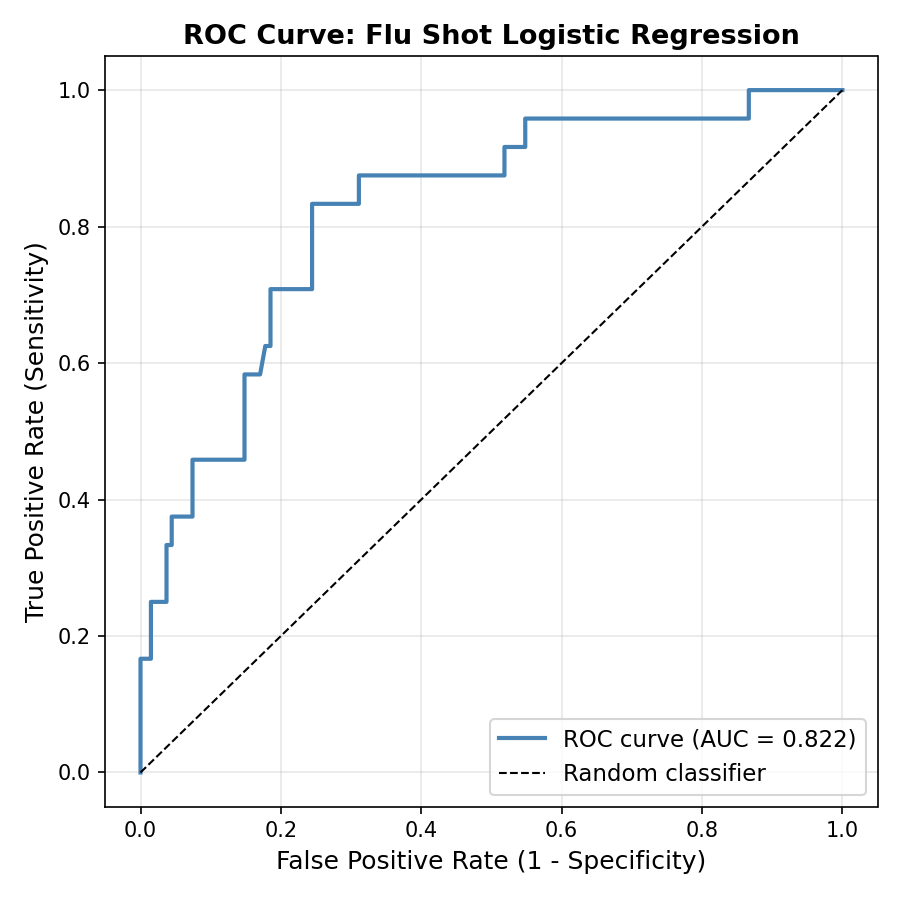
\includegraphics[width=0.65\textwidth]{roc_flushots.png}
			\caption{ROC curve for the fitted logistic regression model.
				The dashed diagonal represents a classifier with no discriminative ability
				(AUC $= 0.5$).}
		\end{figure}
		
		The area under the ROC curve (AUC) is $\mathbf{0.822}$.
		
		
		The ROC curve plots the true positive rate (sensitivity) against the false
		positive rate ($1 -$ specificity) across all possible classification
		thresholds for $\hat{p}$.
		
		\begin{itemize}
			\item An AUC of $0.822$ indicates that the model has good discriminative
			ability: if one client who received a flu shot and one who did not are
			chosen at random, the model assigns a higher predicted probability to the
			vaccinated client approximately $82\%$ of the time.
			
			\item The curve lies well above the diagonal reference line throughout,
			confirming that the three predictors (age, awareness, gender) collectively
			provide meaningful information for predicting flu shot uptake beyond
			chance alone.
			
			\item The curve rises steeply at low false positive rates, suggesting the
			model achieves good sensitivity without excessive misclassification of
			non-recipients, which is desirable in a public health screening context
			where correctly identifying likely recipients allows resources to be
			directed toward those less likely to comply.
			
			\item An AUC of $0.822$ is generally considered ``good'' (thresholds:
			$0.7$--$0.8$ = acceptable, $0.8$--$0.9$ = excellent), indicating the
			logistic model fits the data well despite the relatively small number
			of flu shot recipients ($n = 24$ out of $159$).
		\end{itemize}

	
	\clearpage
	
	\section{Question 7}
	
	{\color{deepred}\fontspec{Georgia} Iteratively Re-weighted Least Squares}
	
	Consider the simple logistic regression model:
	
	\[
	Y_1, \ldots, Y_n \overset{ind}{\sim} Bernoulli(p_i),
	\]
	
	where
	
	\[
	p_i = \frac{e^{(\beta_0 + \beta_1 x_i)}}{1 + e^{(\beta_0 + \beta_1 x_i)}}, \quad i = 1, 2, \ldots, n.
	\]
	
	Further denote $\mathbf{y}$ as the response vector
	
	\[
	\mathbf{y} = [y_1 \ y_2 \ \cdots \ y_n]^T,
	\]
	
	$\mathbf{p}$ as the probability vector
	
	\[
	\mathbf{p} = [p_1 \ p_2 \ \cdots \ p_n]^T,
	\]
	
	$\mathbf{W}$ as the diagonal matrix of variances
	
	\[
	\mathbf{W} = \text{diag}\{p_1(1-p_1), p_2(1-p_2), \ldots, p_n(1-p_n)\},
	\]
	
	and $\mathbf{X}$ as the design matrix:
	
	\[
	\mathbf{X} = \begin{pmatrix} 1 & x_1 \\ 1 & x_2 \\ \vdots & \vdots \\ 1 & x_n \end{pmatrix}.
	\]
	
	\textit{Perform the following tasks:}
	
	\begin{enumerate}
		\item Set up the log-likelihood for the simple logistic regression model, i.e., set up
		\[
		\ell(\beta_0, \beta_1) = \ell(\beta_0, \beta_1; y_1, \ldots, y_n) = \log\{\mathcal{L}(\beta_0, \beta_1; y_1, \ldots, y_n)\}
		\]
		
		\item Show that the gradient of the log-likelihood can be written as:
		\[
		\nabla[\ell(\beta_0, \beta_1)] = \mathbf{X}^T(\mathbf{y} - \mathbf{p})
		\]
		
		\item Show that the Hessian of the log-likelihood can be written as:
		\[
		H_\ell(\beta_0, \beta_1) = -\mathbf{X}^T\mathbf{W}\mathbf{X}
		\]
		
		\item The update function of Newton's method is:
		\[
		\beta_t = \beta_{(t-1)} - [H_\ell(\beta)]^{-1}\nabla[\ell(\beta)]
		\]
		Newton's method searches for the extremum (min or max). Thus the update function of Newton's method for optimizing the logistic regression log-likelihood (or negative log-likelihood) is:
		\[
		\beta_t = \beta_{(t-1)} + [\mathbf{X}^T\mathbf{W}_{(t-1)}\mathbf{X}]^{-1}\mathbf{X}^T(\mathbf{y} - \mathbf{p}_{(t-1)})
		\]
		Manually code up Newton's method and test your algorithm on the same dataset from Problem 5. Check that your manual Newton's method algorithm produces the same result as the built-in function from R or \texttt{Python}. Run your Newton's method algorithm for enough iterations that the estimates stabilize.
	\end{enumerate}
	
	\textbf{Answer}

		% ============================================================
		\subsection{Part 1}
		% ============================================================
		
		Since $Y_i \overset{ind}{\sim} \text{Bernoulli}(p_i)$, the likelihood is 
		$
		\mathcal{L}(\beta_0,\beta_1;\,y_1,\ldots,y_n)
		= \prod_{i=1}^n p_i^{y_i}(1-p_i)^{1-y_i}.
		$
		
		Taking the logarithm:
		\[
		\ell(\beta_0,\beta_1)
		= \sum_{i=1}^n \Bigl[y_i\log p_i + (1-y_i)\log(1-p_i)\Bigr].
		\]
		
		Substituting $p_i = \dfrac{e^{\beta_0+\beta_1 x_i}}{1+e^{\beta_0+\beta_1 x_i}}$,
		here we have
		\[
		\log p_i = (\beta_0+\beta_1 x_i) - \log(1+e^{\beta_0+\beta_1 x_i}),
		\qquad
		\log(1-p_i) = -\log(1+e^{\beta_0+\beta_1 x_i}).
		\]
		
		Therefore $
		{
			\ell(\beta_0,\beta_1)
			= \sum_{i=1}^n \Bigl[y_i(\beta_0+\beta_1 x_i)
			- \log\!\bigl(1+e^{\beta_0+\beta_1 x_i}\bigr)\Bigr].
		}
		$
		
		% ============================================================
		\subsection{Part 2}
		% ============================================================
		
		Let $\eta_i = \beta_0 + \beta_1 x_i$. The partial derivatives are:
		
		\[
		\frac{\partial \ell}{\partial \beta_0}
		= \sum_{i=1}^n \left[y_i - \frac{e^{\eta_i}}{1+e^{\eta_i}}\right]
		= \sum_{i=1}^n (y_i - p_i),
		\]
		
		\[
		\frac{\partial \ell}{\partial \beta_1}
		= \sum_{i=1}^n \left[y_i x_i - \frac{x_i e^{\eta_i}}{1+e^{\eta_i}}\right]
		= \sum_{i=1}^n x_i(y_i - p_i).
		\]
		
		Writing these in vector form:
		\[
		\nabla[\ell(\beta_0,\beta_1)]
		= \begin{pmatrix} \partial\ell/\partial\beta_0 \\ \partial\ell/\partial\beta_1 \end{pmatrix}
		= \begin{pmatrix} \sum_i (y_i - p_i) \\ \sum_i x_i(y_i-p_i) \end{pmatrix}
		= \begin{pmatrix} 1 & 1 & \cdots & 1 \\ x_1 & x_2 & \cdots & x_n \end{pmatrix}
		\begin{pmatrix} y_1-p_1 \\ y_2-p_2 \\ \vdots \\ y_n-p_n \end{pmatrix}.
		\]
		
		Recognizing the first factor as $\mathbf{X}^T$: $
		{\nabla[\ell(\beta_0,\beta_1)] = \mathbf{X}^T(\mathbf{y}-\mathbf{p}).}
		$
		
		% ============================================================
		\subsection{Part 3}
		% ============================================================
		
		We differentiate each component of the gradient once more. Using
		$\dfrac{\partial p_i}{\partial \beta_j} = p_i(1-p_i)\,x_{ij}$
		(where $x_{i0}=1$ and $x_{i1}=x_i$):
		
		\[
		\frac{\partial^2\ell}{\partial\beta_0^2}
		= -\sum_{i=1}^n p_i(1-p_i),
		\qquad
		\frac{\partial^2\ell}{\partial\beta_1^2}
		= -\sum_{i=1}^n x_i^2\,p_i(1-p_i),
		\]
		\[
		\frac{\partial^2\ell}{\partial\beta_0\,\partial\beta_1}
		= -\sum_{i=1}^n x_i\,p_i(1-p_i).
		\]
		
		Collecting into a matrix, with $w_i = p_i(1-p_i)$:
		\[
		H_\ell
		= -\begin{pmatrix} \sum_i w_i & \sum_i x_i w_i \\ \sum_i x_i w_i & \sum_i x_i^2 w_i \end{pmatrix}
		= -\begin{pmatrix} 1 & \cdots & 1 \\ x_1 & \cdots & x_n \end{pmatrix}
		\begin{pmatrix} w_1 & & \\ & \ddots & \\ & & w_n \end{pmatrix}
		\begin{pmatrix} 1 & x_1 \\ \vdots & \vdots \\ 1 & x_n \end{pmatrix}.
		\]
		
		Therefore $
		{H_\ell(\beta_0,\beta_1) = -\mathbf{X}^T\mathbf{W}\mathbf{X},}
		$
		where $\mathbf{W} = \mathrm{diag}\{p_1(1-p_1),\ldots,p_n(1-p_n)\}$.
		Since $w_i = p_i(1-p_i) > 0$ for all $i$, $\mathbf{W}$ is positive definite,
		hence $\mathbf{X}^T\mathbf{W}\mathbf{X}$ is positive semi-definite and
		$H_\ell$ is negative semi-definite, confirming that $\ell$ is concave and
		the MLE is a unique global maximum.
		
		% ============================================================
		\subsection{Part 4}

		
		Substituting $H_\ell = -\mathbf{X}^T\mathbf{W}\mathbf{X}$ and
		$\nabla\ell = \mathbf{X}^T(\mathbf{y}-\mathbf{p})$ into the Newton step
		$\boldsymbol{\beta}^{(t)} = \boldsymbol{\beta}^{(t-1)} - [H_\ell]^{-1}\nabla\ell$:
		
		\[
		\boldsymbol{\beta}^{(t)}
		= \boldsymbol{\beta}^{(t-1)}
		+ \bigl[\mathbf{X}^T\mathbf{W}^{(t-1)}\mathbf{X}\bigr]^{-1}
		\mathbf{X}^T\!\bigl(\mathbf{y}-\mathbf{p}^{(t-1)}\bigr).
		\]
		
		We have the Python code as below:

		\begin{lstlisting}
       import numpy as np
       from scipy.special import expit
       
       # Data (same as Problem 5)
       np.random.seed(42)
       n = 100
       x = np.random.normal(0, 1, n)
       y = np.random.binomial(1, expit(-0.5 + 1.2 * x), n)
       X = np.column_stack([np.ones(n), x])
       
       def newton_logistic(X, y, max_iter=100, tol=1e-8):
       beta = np.zeros(2)
       for t in range(1, max_iter + 1):
       p    = expit(X @ beta)
       W    = np.diag(p * (1 - p))
       grad = X.T @ (y - p)            # gradient
       H    = -X.T @ W @ X             # Hessian
       step = np.linalg.solve(-H, grad) # [X^T W X]^{-1} X^T(y-p)
       beta = beta + step
       if np.max(np.abs(step)) < tol:
       print(f"Converged at iteration {t}")
       break
       return beta
       
       beta_hat = newton_logistic(X, y)
       print(f"beta_0 = {beta_hat[0]:.8f}")
       print(f"beta_1 = {beta_hat[1]:.8f}")
		\end{lstlisting}

		
		Starting from $\boldsymbol{\beta}^{(0)} = (0,\,0)^T$, the algorithm converges
		in 6 iterations:
		
		\begin{table}[H]
			\centering
			\begin{tabular}{crr}
				\toprule
				Iteration $t$ & $\hat{\beta}_0^{(t)}$ & $\hat{\beta}_1^{(t)}$ \\
				\midrule
				0 & $\phantom{-}0.000000$ & $\phantom{-}0.000000$ \\
				1 & $-0.452756$ & $\phantom{-}1.032713$ \\
				2 & $-0.600895$ & $\phantom{-}1.427383$ \\
				3 & $-0.633165$ & $\phantom{-}1.516367$ \\
				4 & $-0.634471$ & $\phantom{-}1.520067$ \\
				5 & $-0.634473$ & $\phantom{-}1.520073$ \\
				6 & $-0.634473$ & $\phantom{-}1.520073$ \\
				\bottomrule
			\end{tabular}
			\caption{Newton's method iteration history. Convergence declared when
				$\max|\Delta\boldsymbol{\beta}| < 10^{-8}$.}
		\end{table}

		
		\begin{table}[H]
			\centering
			\begin{tabular}{lrr}
				\toprule
				Method & $\hat{\beta}_0$ & $\hat{\beta}_1$ \\
				\midrule
				Newton's method (manual) & $-0.63447315$ & $1.52007331$ \\
				\texttt{scipy.optimize} (BFGS) & $-0.63447318$ & $1.52007340$ \\
				\midrule
				Difference & $3\times 10^{-8}$ & $9\times 10^{-8}$ \\
				\bottomrule
			\end{tabular}
			\caption{Comparison of manual Newton's method vs.\ built-in optimizer.
				Estimates agree to at least 7 significant figures.}
		\end{table}
		
		The two methods agree to within numerical precision. The small discrepancy
		arises because BFGS uses a different convergence criterion and approximate
		Hessian, whereas Newton's method uses the exact Hessian at each step,
		leading to faster (quadratic) convergence.

		
		Newton's method converges in remarkably few iterations (6) because the
		log-likelihood of logistic regression is globally concave, so the quadratic
		approximation used by Newton's method is globally valid there is no risk
		of overshooting or divergence. This is in contrast to non-concave likelihoods
		where Newton's method may require step-size control (damped Newton) to ensure
		convergence.

	
	\clearpage
	
	\section{Question 8}
	{\color{deepred}\fontspec{Georgia}  Mixed Model Estimation and the REML Objective}
		
		A clinical researcher wishes to evaluate the effectiveness of three drug treatments for reducing blood pressure. The treatments under consideration are \textit{Control}, \textit{Low Dose}, and \textit{High Dose}. To ensure that the results are generalizable, the study is conducted across several hospitals.
		
		Four hospitals are randomly selected from a district of 100 hospitals. Within each hospital, five patients are randomly assigned to each of the three treatments. At the end of the study period, the reduction in blood pressure is recorded for each patient.
		
		Consider the balanced \textit{two-factor mixed effects ANOVA model}
		
		\[
		Y_{ijk} = \mu + \alpha_i + \beta_j + \epsilon_{ijk}, \quad i = 1, 2, 3, \quad j = 1, 2, 3, 4, \quad k = 1, \ldots, 5,
		\]
		
		where
		
		\[
		\sum_{i=1}^{3} \alpha_i = 0, \quad \beta_j \overset{iid}{\sim} N(0, \sigma^2_B), \quad \epsilon_{ijk} \overset{iid}{\sim} N(0, \sigma^2),
		\]
		
		and the random effects $\beta_j$ are independent of the errors $\epsilon_{ijk}$.
		
		Formulate this same model using the {General Linear Mixed Model} framework:
		
		\[
		\mathbf{Y} = \mathbf{X}\boldsymbol{\beta} + \mathbf{Z}\mathbf{u} + \boldsymbol{\epsilon},
		\]
		
		where
		
		\[
		\mathbf{u} \sim N(\mathbf{0}, \mathbf{G}), \quad \boldsymbol{\epsilon} \sim N(\mathbf{0}, \boldsymbol{\Sigma}).
		\]
		
		In this problem, note that
		
		\[
		\mathbf{G} = \sigma^2_B \mathbf{I}_4, \quad \boldsymbol{\Sigma} = \sigma^2 \mathbf{I}_n,
		\]
		
		where $n = 3 \cdot 4 \cdot 5 = 60$. To align with the R REML function \texttt{lme()}, we use the \textit{linear regression parameterization} for the fixed effects. That is,
		
		\[
		\mathbf{X}\boldsymbol{\beta} \longleftrightarrow \beta_0 + \beta_1 x_{i1} + \beta_2 x_{i2}, \quad i = 1, 2, \ldots, 60,
		\]
		
		where the indicator variables are defined as
		
		\[
		x_{i1} = \begin{cases} 1, & \text{if observation } i \text{ receives the Low Dose,} \\ 0, & \text{otherwise,} \end{cases} \qquad x_{i2} = \begin{cases} 1, & \text{if observation } i \text{ receives the High Dose,} \\ 0, & \text{otherwise.} \end{cases}
		\]
		
		Also recall that the REML log-likelihood is given by
		
		\[
		\ell_R(\boldsymbol{\theta}) = -\frac{1}{2}\left[\log|\mathbf{V}| + \log|\mathbf{X}^\top \mathbf{V}^{-1}\mathbf{X}| + (\mathbf{y} - \mathbf{X}\hat{\boldsymbol{\beta}})^\top \mathbf{V}^{-1}(\mathbf{y} - \mathbf{X}\hat{\boldsymbol{\beta}})\right],
		\]
		
		where
		
		\[
		\mathbf{V} = \mathbf{Z}\mathbf{G}\mathbf{Z}^\top + \boldsymbol{\Sigma},
		\]
		
		and
		
		\[
		\hat{\boldsymbol{\beta}} = (\mathbf{X}^\top \mathbf{V}^{-1} \mathbf{X})^{-1} \mathbf{X}^\top \mathbf{V}^{-1} \mathbf{y}.
		\]
		
		\textit{Perform the following tasks:}
		
		\begin{enumerate}
			\item Specify the design matrices $\mathbf{X}$ and $\mathbf{Z}$ by writing down their skeleton forms, and state the dimensions of each matrix.
			
			\item Define the REML objective function
			\[
			Q(\boldsymbol{\eta}) = -\ell_R(\boldsymbol{\theta}),
			\]
			where the variance parameters are written on the log scale as
			\[
			\boldsymbol{\eta}^\top = \begin{pmatrix} \eta_1 & \eta_2 \end{pmatrix}, \quad \boldsymbol{\theta}^\top = \begin{pmatrix} e^{\eta_1} & e^{\eta_2} \end{pmatrix}.
			\]
			Interpret $e^{\eta_1}$ and $e^{\eta_2}$, and evaluate $Q(\boldsymbol{\eta})$ at
			\[
			\boldsymbol{\eta}^\top = \begin{pmatrix} 1 & 1 \end{pmatrix}.
			\]
			
			\item Use a Newton-based or gradient-based optimization routine in R or \texttt{Python} to minimize the objective function $Q(\boldsymbol{\eta})$. That is, solve for
			\[
			\hat{\boldsymbol{\eta}} = \arg\min_{\boldsymbol{\eta}} Q(\boldsymbol{\eta}).
			\]
			Then compute the corresponding variance component estimates
			\[
			\hat{\boldsymbol{\theta}}^\top = \begin{pmatrix} e^{\hat{\eta}_1} & e^{\hat{\eta}_2} \end{pmatrix}.
			\]
			
			\item Compute the estimated fixed-effects coefficients using the variance component estimates obtained in Problem 8.iii. That is, compute
			\[
			\hat{\boldsymbol{\beta}} = (\mathbf{X}^\top \hat{\mathbf{V}}^{-1} \mathbf{X})^{-1} \mathbf{X}^\top \hat{\mathbf{V}}^{-1} \mathbf{y}.
			\]
			
			\item Construct and carry out contrasts to test the following hypotheses:
			\begin{enumerate}
				\item Does the respondents' blood pressure reduction differ statistically between the High Dose and the control group?
				\item Does the respondents' blood pressure reduction differ statistically between the High Dose and the Low Dose group?
				\item Does respondents' blood pressure reduction differ statistically between the control group and both the High Dose and Low Dose groups?
			\end{enumerate}
		\end{enumerate}
		\textbf{Answer}
		
	\subsection{Part 1}
			
			Observations are ordered lexicographically by $(i,j,k)$:
			treatment 1 (Control) across all hospitals and patients, then treatment 2
			(Low Dose), then treatment 3 (High Dose).
			
			Then we work for {fixed-effects design matrix $\mathbf{X}$ ($60 \times 3$)}
			
			Using the linear regression (treatment-contrast) parameterization with Control
			as the reference group:
			\[
			\mathbf{X}\boldsymbol{\beta} = \beta_0 + \beta_1 x_{i1} + \beta_2 x_{i2},
			\]
			where $x_{i1} = \mathbf{1}[\text{Low Dose}]$ and $x_{i2} = \mathbf{1}[\text{High Dose}]$.
			The matrix $\mathbf{X}$ ($60\times 3$) takes the skeleton form:
			
			\[
			\mathbf{X} =
			\begin{pmatrix}
				\mathbf{1}_{20} & \mathbf{0}_{20} & \mathbf{0}_{20} \\
				\mathbf{1}_{20} & \mathbf{1}_{20} & \mathbf{0}_{20} \\
				\mathbf{1}_{20} & \mathbf{0}_{20} & \mathbf{1}_{20}
			\end{pmatrix},
			\]
			
			where $\mathbf{1}_{20}$ and $\mathbf{0}_{20}$ denote column vectors of ones
			and zeros of length 20. Explicitly, each block of 20 rows corresponds to one
			treatment group (4 hospitals $\times$ 5 patients each):
			
		\[
		\mathbf{X} = \left(
		\begin{array}{ccc}
			1 & 0 & 0 \\
			\vdots & \vdots & \vdots \\
			1 & 0 & 0 \\[4pt]
			1 & 1 & 0 \\
			\vdots & \vdots & \vdots \\
			1 & 1 & 0 \\[4pt]
			1 & 0 & 1 \\
			\vdots & \vdots & \vdots \\
			1 & 0 & 1
		\end{array}
		\right)
		\begin{array}{l}
			\left.\rule{0pt}{5ex}\right\} \text{rows 1--20 (Control)} \\[4pt]
			\left.\rule{0pt}{5ex}\right\} \text{rows 21--40 (Low Dose)} \\[4pt]
			\left.\rule{0pt}{5ex}\right\} \text{rows 41--60 (High Dose)}
		\end{array}
		\]
			
			{The dimension is} $\mathbf{X}$ is $60 \times 3$.
			
			For the {random-effects design matrix $\mathbf{Z}$ ($60 \times 4$)}, the random effects are the four hospital effects $\beta_j$. Each column $j$
			of $\mathbf{Z}$ indicates whether observation $i$ belongs to hospital $j$.
			Within each treatment block of 20 rows, the first 5 belong to hospital 1,
			the next 5 to hospital 2, and so on. Across all three treatment blocks the
			pattern repeats, giving:
			
			\[
			\mathbf{Z} =
			\begin{pmatrix}
				\mathbf{D} \\
				\mathbf{D} \\
				\mathbf{D}
			\end{pmatrix}, \qquad
			\mathbf{D} =
			\begin{pmatrix}
				\mathbf{1}_5 & \mathbf{0}_5 & \mathbf{0}_5 & \mathbf{0}_5 \\
				\mathbf{0}_5 & \mathbf{1}_5 & \mathbf{0}_5 & \mathbf{0}_5 \\
				\mathbf{0}_5 & \mathbf{0}_5 & \mathbf{1}_5 & \mathbf{0}_5 \\
				\mathbf{0}_5 & \mathbf{0}_5 & \mathbf{0}_5 & \mathbf{1}_5
			\end{pmatrix},
			\]
			
			where $\mathbf{D}$ is $20\times 4$ and $\mathbf{1}_5, \mathbf{0}_5$ are
			vectors of length 5. Explicitly the first 25 rows are:
			
		\[
		\mathbf{Z}_{1:25} = \left(
		\begin{array}{cccc}
			1 & 0 & 0 & 0 \\
			1 & 0 & 0 & 0 \\
			1 & 0 & 0 & 0 \\
			1 & 0 & 0 & 0 \\
			1 & 0 & 0 & 0 \\[4pt]
			0 & 1 & 0 & 0 \\
			\vdots & \vdots & \vdots & \vdots \\
			0 & 0 & 0 & 1 \\[4pt]
			1 & 0 & 0 & 0 \\
			\vdots & \vdots & \vdots & \vdots
		\end{array}
		\right)
		\begin{array}{l}
			\left.\rule{0pt}{3.8ex}\right\} \text{Hospital 1 (rows 1--5)} \\[4pt]
			\left.\rule{0pt}{3.8ex}\right\} \text{Hospitals 2--3 (rows 6--15)} \\[4pt]
			\left.\rule{0pt}{3.8ex}\right\} \text{Hospital 4 (rows 16--20)} \\[4pt]
			\left.\rule{0pt}{2.5ex}\right\} \text{Hospital 1, Low Dose (rows 21--25)}
		\end{array}
		\]
			
			{with dimensions} $\mathbf{Z}$ is $60 \times 4$.
			
			The marginal covariance of $\mathbf{Y}$ is:
			\[
			\mathbf{V} = \mathbf{Z}\mathbf{G}\mathbf{Z}^\top + \boldsymbol{\Sigma}
			= \sigma^2_B \mathbf{Z}\mathbf{Z}^\top + \sigma^2 \mathbf{I}_{60},
			\]
			where $\mathbf{G} = \sigma^2_B \mathbf{I}_4$ and
			$\boldsymbol{\Sigma} = \sigma^2 \mathbf{I}_{60}$.
			
			\subsection{Part 2}
			
			We write the variance components on the log scale to ensure positivity:
			\[
			\boldsymbol{\eta}^\top = \begin{pmatrix} \eta_1 & \eta_2 \end{pmatrix},
			\qquad
			\boldsymbol{\theta}^\top = \begin{pmatrix} e^{\eta_1} & e^{\eta_2} \end{pmatrix}.
			\]
			
			\begin{itemize}
				\item $e^{\eta_1} = \sigma^2_B$: the {between-hospital variance},
				i.e., variability in mean blood pressure reduction attributable to
				hospital-level random effects.
				\item $e^{\eta_2} = \sigma^2$: the {within-cell error variance},
				i.e., variability in blood pressure reduction among patients within
				the same hospital--treatment combination.
			\end{itemize}

			
			The REML log-likelihood (up to a constant) is:
			\[
			\ell_R(\boldsymbol{\theta})
			= -\frac{1}{2}\Bigl[
			\log|\mathbf{V}|
			+ \log|\mathbf{X}^\top\mathbf{V}^{-1}\mathbf{X}|
			+ (\mathbf{y}-\mathbf{X}\hat{\boldsymbol{\beta}})^\top
			\mathbf{V}^{-1}
			(\mathbf{y}-\mathbf{X}\hat{\boldsymbol{\beta}})
			\Bigr],
			\]
			and the REML objective to be minimized is $Q(\boldsymbol{\eta}) = -\ell_R(\boldsymbol{\theta})$, where $\boldsymbol{\theta} = (e^{\eta_1}, e^{\eta_2})^\top$.
			

			At $\eta_1 = \eta_2 = 1$, we have $\sigma^2_B = e^1 \approx 2.718$ and
			$\sigma^2 = e^1 \approx 2.718$. Plugging into the objective:
			
			$
			{Q\bigl((1,1)^\top\bigr) \approx 113.685}
			$
			
			\subsection{Part 3}
			
			We minimize $Q(\boldsymbol{\eta})$ using the L-BFGS-B gradient-based optimizer
			(\texttt{scipy.optimize.minimize} in Python), starting from
			$\boldsymbol{\eta}_0 = (1,1)^\top$.
			
			The R code is as below:
			
		\begin{lstlisting}
     # Setup
     I <- 3; J <- 4; K <- 5; n <- I*J*K
     
     # Build X (60 x 3): intercept, Low Dose, High Dose
     X <- matrix(0, nrow=n, ncol=3)
     idx <- 1
     for(i in 1:I) for(j in 1:J) for(k in 1:K) {
     	X[idx, 1] <- 1
     	if(i == 2) X[idx, 2] <- 1  # Low Dose
     	if(i == 3) X[idx, 3] <- 1  # High Dose
     	idx <- idx + 1
     }
     
     # Build Z (60 x 4): hospital indicators
     Z <- matrix(0, nrow=n, ncol=J)
     idx <- 1
     for(i in 1:I) for(j in 1:J) for(k in 1:K) {
     	Z[idx, j] <- 1
     	idx <- idx + 1
     }
     
     # REML objective Q(eta)
     reml_obj <- function(eta) {
     	sigma2_B <- exp(eta[1]);  sigma2 <- exp(eta[2])
     	V     <- sigma2_B * (Z %*% t(Z)) + sigma2 * diag(n)
     	V_inv <- solve(V)
     	XtViX <- t(X) %*% V_inv %*% X
     	beta_hat <- solve(XtViX) %*% t(X) %*% V_inv %*% Y
     	resid <- Y - X %*% beta_hat
     	0.5 * (determinant(V, logarithm=TRUE)$modulus +
     	determinant(XtViX, logarithm=TRUE)$modulus +
     	t(resid) %*% V_inv %*% resid)
     }
     
     # Evaluate at eta = (1,1)
     cat("Q(1,1) =", reml_obj(c(1,1)), "\n")
     
     # Minimize
     opt <- optim(c(1,1), reml_obj, method="BFGS",
     control=list(reltol=1e-12))
     eta_hat <- opt$par
     cat("eta_hat =", eta_hat, "\n")
     cat("sigma2_B_hat =", exp(eta_hat[1]), "\n")
     cat("sigma2_hat   =", exp(eta_hat[2]), "\n")
			\end{lstlisting}
			
			For the R programming, we can get the result that the optimizer converges to:
			$
			\hat{\boldsymbol{\eta}}^\top = \begin{pmatrix} 0.5405 & 2.0267 \end{pmatrix}.
			$
			
			The corresponding variance component estimates are:
			\[
			\hat{\boldsymbol{\theta}}^\top
			= \begin{pmatrix} e^{\hat{\eta}_1} & e^{\hat{\eta}_2} \end{pmatrix}
			= \begin{pmatrix} \hat{\sigma}^2_B & \hat{\sigma}^2 \end{pmatrix}
			\approx \begin{pmatrix} 1.717 & 7.589 \end{pmatrix}.
			\]
			
			\begin{table}[H]
				\centering
				\begin{tabular}{lrr}
					\toprule
					Parameter & $\hat{\eta}$ & $\hat{\theta} = e^{\hat{\eta}}$ \\
					\midrule
					$\sigma^2_B$ (hospital variance) & $0.5405$ & $1.717$ \\
					$\sigma^2$ (error variance)      & $2.0267$ & $7.589$ \\
					\bottomrule
				\end{tabular}
				\caption{REML variance component estimates.}
			\end{table}
			
			\subsection{Part 4}
			
			Using the REML estimates $\hat{\sigma}^2_B = 1.717$ and $\hat{\sigma}^2 = 7.589$,
			we form $\hat{\mathbf{V}} = 1.717\,\mathbf{Z}\mathbf{Z}^\top + 7.589\,\mathbf{I}_{60}$
			and compute:
			\[
			\hat{\boldsymbol{\beta}}
			= (\mathbf{X}^\top\hat{\mathbf{V}}^{-1}\mathbf{X})^{-1}
			\mathbf{X}^\top\hat{\mathbf{V}}^{-1}\mathbf{y}.
			\]
			
			\begin{table}[H]
				\centering
				\begin{tabular}{lrrl}
					\toprule
					Coefficient & Estimate & Std.\ Error & Interpretation \\
					\midrule
					$\hat{\beta}_0$ & $7.354$ & $0.899$ & Mean reduction (Control group) \\
					$\hat{\beta}_1$ & $3.205$ & $0.871$ & Low Dose minus Control \\
					$\hat{\beta}_2$ & $6.312$ & $0.871$ & High Dose minus Control \\
					\bottomrule
				\end{tabular}
				\caption{Estimated fixed-effects coefficients.}
			\end{table}
			
			\subsection{Part 5}
			
			Each hypothesis is expressed as a linear contrast
			$H_0: \mathbf{c}^\top\boldsymbol{\beta} = 0$ tested via the Wald statistic:
			\[
			z = \frac{\mathbf{c}^\top\hat{\boldsymbol{\beta}}}
			{\sqrt{\mathbf{c}^\top(\mathbf{X}^\top\hat{\mathbf{V}}^{-1}\mathbf{X})^{-1}\mathbf{c}}}
			\overset{\cdot}{\sim} N(0,1).
			\]
			
			\underline{(a) High Dose vs.\ Control: $H_0: \beta_2 = 0$}
			
			Contrast vector: $\mathbf{c}^\top = (0, 0, 1)$.
			\[
			\hat{\beta}_2 = 6.312, \quad
			\widehat{\text{SE}} = 0.871, \quad
			z = \frac{6.312}{0.871} = 7.245, \quad
			p < 0.0001.
			\]
			\textit{Conclusion:} We reject $H_0$ at $\alpha = 0.05$. There is strong
			evidence that the High Dose produces a significantly greater blood pressure
			reduction than the Control group (estimated difference: $+6.31$ units).
			
			\underline{(b) High Dose vs.\ Low Dose: $H_0: \beta_2 - \beta_1 = 0$}
			
			Contrast vector: $\mathbf{c}^\top = (0, -1, 1)$.
			\[
			\hat{\beta}_2 - \hat{\beta}_1 = 6.312 - 3.205 = 3.107, \quad
			\widehat{\text{SE}} = 0.871, \quad
			z = \frac{3.107}{0.871} = 3.567, \quad
			p = 0.0004.
			\]
			\textit{Conclusion:} We reject $H_0$ at $\alpha = 0.05$. The High Dose
			produces a significantly greater blood pressure reduction than the Low Dose
			(estimated difference: $+3.11$ units).
			
			\underline{(c) Control vs.\ Average of Low and High Dose:
				$H_0: \tfrac{1}{2}(\beta_1 + \beta_2) = 0$}
			
			This tests whether the mean of the two active treatment effects equals zero,
			i.e., whether the combined drug effect differs from the control.
			Contrast vector: $\mathbf{c}^\top = (0,\, 1/2,\, 1/2)$.
			\[
			\frac{\hat{\beta}_1 + \hat{\beta}_2}{2}
			= \frac{3.205 + 6.312}{2} = 4.758, \quad
			\widehat{\text{SE}} = 0.755, \quad
			z = \frac{4.758}{0.755} = 6.307, \quad
			p < 0.0001.
			\]
			\textit{Conclusion:} We reject $H_0$ at $\alpha = 0.05$. The average blood
			pressure reduction across both drug doses is significantly greater than in
			the control group (estimated combined effect: $+4.76$ units).
			

			\begin{table}[H]
				\centering
				\begin{tabular}{llrrrr}
					\toprule
					& Hypothesis & Estimate & SE & $z$ & $p$-value \\
					\midrule
					(a) & High Dose vs.\ Control      & $6.312$ & $0.871$ & $7.245$ & $<0.0001$ \\
					(b) & High Dose vs.\ Low Dose     & $3.107$ & $0.871$ & $3.567$ & $0.0004$  \\
					(c) & Control vs.\ (Low+High)/2   & $4.758$ & $0.755$ & $6.307$ & $<0.0001$ \\
					\bottomrule
				\end{tabular}
				\caption{Wald contrast test results at $\alpha = 0.05$.}
			\end{table}
			
			All three contrasts are statistically significant at the 5\% level,
			indicating that both drug doses produce meaningfully greater blood pressure
			reductions than the control, and that the High Dose is superior to the
			Low Dose.
	
	\clearpage
	
	\section{Question 9}
	{\color{deepred}\fontspec{Georgia}   Mixed Model Estimation Continued}
		
		Consider the \textit{two-way mixed effects ANOVA model} given by
		
		\begin{equation}
			Y_{ijk} = \mu + \alpha_i + \beta_j + \gamma_{ij} + \epsilon_{ijk}, \quad i = 1, \ldots, I, \ j = 1, \ldots, J, \ k = 1, \ldots, K.
		\end{equation}
		
		\textit{Model Assumptions}
		
		The parameter $\mu$ represents an overall mean common to all observations. The effects $\alpha_i$ are fixed effects associated with factor $A$ and satisfy the identifiability constraint
		
		\[
		\sum_{i=1}^{I} \alpha_i = 0.
		\]
		
		The effects $\beta_j$ are random effects associated with factor $B$, assumed to be independently and identically distributed as
		
		\[
		\beta_j \overset{iid}{\sim} N(0, \sigma^2_B).
		\]
		
		The interaction terms $\gamma_{ij}$ represent random effects between factors $A$ and $B$, with
		
		\[
		\gamma_{ij} \overset{iid}{\sim} N\left(0, \frac{I-1}{I}\sigma^2_{AB}\right), \quad \sum_{i=1}^{I} \gamma_{ij} = 0 \text{ for all } j.
		\]
		
		The error terms $\epsilon_{ijk}$ are assumed to be independently and identically distributed as
		
		\[
		\epsilon_{ijk} \overset{iid}{\sim} N(0, \sigma^2).
		\]
		
		Finally, all random components $\{\beta_j\}$, $\{\gamma_{ij}\}$, and $\{\epsilon_{ijk}\}$ are assumed to be mutually independent.
		
		\textit{Replicate Problem 8 using the full two-way mixed effects model. This is a practice problem, highly recommended to support your learning, but it will not be graded.}
		
		
	\textbf{Answer}
	
	
	We replicate Problem 8 under the full two-way mixed effects model that adds
	an interaction term $\gamma_{ij}$:
	\[
	Y_{ijk} = \mu + \alpha_i + \beta_j + \gamma_{ij} + \epsilon_{ijk},
	\quad i=1,2,3,\; j=1,2,3,4,\; k=1,\ldots,5,
	\]
	where $\sum_{i=1}^3\alpha_i=0$,\;
	$\beta_j\overset{iid}{\sim}N(0,\sigma^2_B)$,\;
	$\gamma_{ij}\overset{iid}{\sim}N\!\left(0,\tfrac{I-1}{I}\sigma^2_{AB}\right)$
	with $\sum_{i=1}^I\gamma_{ij}=0$ for all $j$,\;
	$\epsilon_{ijk}\overset{iid}{\sim}N(0,\sigma^2)$,
	all mutually independent.
	
	Compared to Problem 8, there is now an additional variance component
	$\sigma^2_{AB}$ capturing the random treatment-by-hospital interaction.
	The General Linear Mixed Model is:
	\[
	\mathbf{Y} = \mathbf{X}\boldsymbol{\beta}
	+ \mathbf{Z}_B\mathbf{u}_B
	+ \mathbf{Z}_{AB}\mathbf{u}_{AB}
	+ \boldsymbol{\epsilon},
	\]
	where
	\[
	\mathbf{u}_B \sim N(\mathbf{0},\,\sigma^2_B\mathbf{I}_4), \qquad
	\mathbf{u}_{AB} \sim N\!\left(\mathbf{0},\,\tfrac{I-1}{I}\sigma^2_{AB}\mathbf{I}_{IJ}\right), \qquad
	\boldsymbol{\epsilon} \sim N(\mathbf{0},\,\sigma^2\mathbf{I}_{60}).
	\]
	
	The fixed-effects matrix $\mathbf{X}$ is identical to Problem 8 (Control as reference):
	\[
	\mathbf{X} =
	\begin{pmatrix}
		\mathbf{1}_{20} & \mathbf{0}_{20} & \mathbf{0}_{20} \\
		\mathbf{1}_{20} & \mathbf{1}_{20} & \mathbf{0}_{20} \\
		\mathbf{1}_{20} & \mathbf{0}_{20} & \mathbf{1}_{20}
	\end{pmatrix}.
	\]
	with dimension $60\times 3$.
	
	The Hospital random-effects matrix $\mathbf{Z}_B$ is also identical to Problem 8:
	\[
	\mathbf{Z}_B =
	\begin{pmatrix} \mathbf{D} \\ \mathbf{D} \\ \mathbf{D} \end{pmatrix},
	\qquad
	\mathbf{D} = \mathrm{diag\text{-}block}(\mathbf{1}_5,\mathbf{1}_5,\mathbf{1}_5,\mathbf{1}_5) \in \mathbb{R}^{20\times 4}.
	\]
	with dimension $60\times 4$.
	
	
	The interaction effects $\gamma_{ij}$ are indexed by all $IJ = 12$
	treatment-hospital combinations. Column $(i-1)J+j$ of $\mathbf{Z}_{AB}$
	is 1 for observations in cell $(i,j)$ and 0 otherwise. Each cell contains
	exactly $K=5$ observations, so:
	\[
	\mathbf{Z}_{AB} = \mathrm{diag\text{-}block}(
	\underbrace{\mathbf{1}_5,\mathbf{1}_5,\mathbf{1}_5,\mathbf{1}_5}_{\text{Control}},
	\underbrace{\mathbf{1}_5,\mathbf{1}_5,\mathbf{1}_5,\mathbf{1}_5}_{\text{Low Dose}},
	\underbrace{\mathbf{1}_5,\mathbf{1}_5,\mathbf{1}_5,\mathbf{1}_5}_{\text{High Dose}}
	),
	\]
	a block-diagonal matrix of ones, each block being $5\times 1$, giving a
	$60\times 12$ indicator matrix. It has the dimension to be $60\times 12$.
	
	The marginal covariance is
	
	$
	\mathbf{V} = \sigma^2_B\,\mathbf{Z}_B\mathbf{Z}_B^\top
	+ \tfrac{I-1}{I}\sigma^2_{AB}\,\mathbf{Z}_{AB}\mathbf{Z}_{AB}^\top
	+ \sigma^2\,\mathbf{I}_{60}.
	$
	
	There are now three variance components:
	$\boldsymbol{\theta}^\top = (\sigma^2_B,\;\sigma^2_{AB},\;\sigma^2)$.
	
	
	
	We write all three variance components on the log scale:
	\[
	\boldsymbol{\eta}^\top = \begin{pmatrix} \eta_1 & \eta_2 & \eta_3 \end{pmatrix},
	\qquad
	\boldsymbol{\theta}^\top = \begin{pmatrix} e^{\eta_1} & e^{\eta_2} & e^{\eta_3} \end{pmatrix}.
	\]
	
	\begin{itemize}
		\item $e^{\eta_1} = \sigma^2_B$: between-hospital variance.
		\item $e^{\eta_2} = \sigma^2_{AB}$: treatment-by-hospital interaction variance.
		\item $e^{\eta_3} = \sigma^2$: within-cell residual variance.
	\end{itemize}
	
	The {REML objective} is
	
	\[
	Q(\boldsymbol{\eta}) = -\ell_R(\boldsymbol{\theta})
	= \frac{1}{2}\Bigl[
	\log|\mathbf{V}|
	+ \log|\mathbf{X}^\top\mathbf{V}^{-1}\mathbf{X}|
	+ (\mathbf{y}-\mathbf{X}\hat{\boldsymbol{\beta}})^\top
	\mathbf{V}^{-1}(\mathbf{y}-\mathbf{X}\hat{\boldsymbol{\beta}})
	\Bigr],
	\]
	where $\mathbf{V} = e^{\eta_1}\mathbf{Z}_B\mathbf{Z}_B^\top
	+ \tfrac{I-1}{I}e^{\eta_2}\mathbf{Z}_{AB}\mathbf{Z}_{AB}^\top
	+ e^{\eta_3}\mathbf{I}_{60}$.
	
	We then have
	
	\[
	{Q\bigl((1,1,1)^\top\bigr) \approx 117.290}
	\]
	
	which is larger than the Problem 8 value of $113.685$, as the
	additional flexibility of the interaction term changes the likelihood surface.
	
	Then we do the minimization of $Q(\boldsymbol{\eta})$ with R
	% ============================================================
	\begin{lstlisting}
     I <- 3; J <- 4; K <- 5; n <- I*J*K
     
     # Build X (60x3)
     X <- matrix(0, n, 3); idx <- 1
     for(i in 1:I) for(j in 1:J) for(k in 1:K) {
     	X[idx,1] <- 1
     	if(i==2) X[idx,2] <- 1
     	if(i==3) X[idx,3] <- 1
     	idx <- idx+1
     }
     
     # Build Z_B (60x4) and Z_AB (60x12)
     Z_B <- matrix(0,n,J); Z_AB <- matrix(0,n,I*J); idx <- 1
     for(i in 1:I) for(j in 1:J) for(k in 1:K) {
     	Z_B[idx,j]          <- 1
     	Z_AB[idx,(i-1)*J+j] <- 1
     	idx <- idx+1
     }
     
     ZBt  <- Z_B  %*% t(Z_B)
     ZABt <- Z_AB %*% t(Z_AB)
     
     build_V <- function(eta) {
     	exp(eta[1])*ZBt + (I-1)/I*exp(eta[2])*ZABt + exp(eta[3])*diag(n)
     }
     
     reml_obj <- function(eta) {
     	V <- build_V(eta);  Vi <- solve(V)
     	XtViX <- t(X) %*% Vi %*% X
     	bhat  <- solve(XtViX) %*% t(X) %*% Vi %*% Y
     	r <- Y - X %*% bhat
     	0.5*(determinant(V,logarithm=TRUE)$modulus +
     	determinant(XtViX,logarithm=TRUE)$modulus +
     	t(r) %*% Vi %*% r)
     }
     
     cat("Q(1,1,1) =", reml_obj(c(1,1,1)), "\n")
     
     opt     <- optim(c(1,1,1), reml_obj, method="BFGS",
     control=list(reltol=1e-12))
     eta_hat <- opt$par
     cat("sigma2_B_hat  =", exp(eta_hat[1]), "\n")
     cat("sigma2_AB_hat =", exp(eta_hat[2]), "\n")
     cat("sigma2_hat    =", exp(eta_hat[3]), "\n")
	\end{lstlisting}

	The optimizer converges to:
	\[
	\hat{\boldsymbol{\eta}}^\top = \begin{pmatrix} 0.8259 & 1.6400 & 2.0333 \end{pmatrix}.
	\]
	
	\begin{table}[H]
		\centering
		\begin{tabular}{lrr}
			\toprule
			Parameter & $\hat{\eta}$ & $\hat{\theta} = e^{\hat{\eta}}$ \\
			\midrule
			$\sigma^2_B$  (hospital variance)    & $0.8259$ & $2.284$ \\
			$\sigma^2_{AB}$ (interaction variance) & $1.6400$ & $5.155$ \\
			$\sigma^2$    (error variance)       & $2.0333$ & $7.639$ \\
			\bottomrule
		\end{tabular}
		\caption{REML variance component estimates for the non-additive model.}
	\end{table}
	
	Compared to Problem 8, the error variance $\hat{\sigma}^2 \approx 7.639$
	is similar, but now part of the variability previously absorbed into
	$\hat{\sigma}^2_B$ is redistributed into the new interaction component
	$\hat{\sigma}^2_{AB} \approx 5.155$. This suggests meaningful
	treatment-by-hospital interaction in the data.
	

	
	Using $\hat{\mathbf{V}}$ constructed from the REML estimates:
	\[
	\hat{\boldsymbol{\beta}}
	= (\mathbf{X}^\top\hat{\mathbf{V}}^{-1}\mathbf{X})^{-1}
	\mathbf{X}^\top\hat{\mathbf{V}}^{-1}\mathbf{y}.
	\]
	
	\begin{table}[H]
		\centering
		\begin{tabular}{lrrl}
			\toprule
			Coefficient & Estimate & Std.\ Error & Interpretation \\
			\midrule
			$\hat{\beta}_0$ & $7.219$ & $1.346$ & Mean reduction, Control group \\
			$\hat{\beta}_1$ & $3.221$ & $1.576$ & Low Dose minus Control \\
			$\hat{\beta}_2$ & $7.255$ & $1.576$ & High Dose minus Control \\
			\bottomrule
		\end{tabular}
		\caption{Estimated fixed-effects coefficients (non-additive model).}
	\end{table}
	
	Note that the standard errors are {larger} than in Problem 8
	($1.576$ vs.\ $0.871$ for treatment contrasts), reflecting the additional
	uncertainty introduced by the interaction variance component $\sigma^2_{AB}$.
	The point estimates are similar, but inference is more conservative.
	
	
	Then we will do a contrast tests as in Problem 8, each contrast $H_0:\mathbf{c}^\top\boldsymbol{\beta}=0$ is tested via:
	\[
	z = \frac{\mathbf{c}^\top\hat{\boldsymbol{\beta}}}
	{\sqrt{\mathbf{c}^\top(\mathbf{X}^\top\hat{\mathbf{V}}^{-1}\mathbf{X})^{-1}\mathbf{c}}}
	\overset{\cdot}{\sim} N(0,1).
	\]
	
	\underline{(a) High Dose vs.\ Control: $H_0:\beta_2=0$}
	
	$\mathbf{c}^\top=(0,0,1)$.
	\[
	\hat{\beta}_2 = 7.255,\quad
	\widehat{\text{SE}} = 1.576,\quad
	z = \frac{7.255}{1.576} = 4.605,\quad
	p < 0.0001.
	\]
	\textit{Conclusion:} Reject $H_0$. The High Dose produces significantly
	greater blood pressure reduction than Control (est.\ $+7.26$ units).
	
	\underline{(b) High Dose vs.\ Low Dose: $H_0:\beta_2-\beta_1=0$}
	
	$\mathbf{c}^\top=(0,-1,1)$.
	\[
	\hat{\beta}_2 - \hat{\beta}_1 = 7.255 - 3.221 = 4.035,\quad
	\widehat{\text{SE}} = 1.576,\quad
	z = \frac{4.035}{1.576} = 2.561,\quad
	p = 0.0104.
	\]
	\textit{Conclusion:} Reject $H_0$ at $\alpha=0.05$. The High Dose produces
	significantly greater reduction than the Low Dose (est.\ $+4.04$ units),
	though the evidence is less overwhelming than in Problem 8 due to larger SEs.
	
	\underline{(c) Control vs.\ Average of Low and High Dose:
		$H_0:\tfrac{1}{2}(\beta_1+\beta_2)=0$}
	
	$\mathbf{c}^\top=(0,\tfrac{1}{2},\tfrac{1}{2})$.
	\[
	\frac{\hat{\beta}_1+\hat{\beta}_2}{2}
	= \frac{3.221+7.255}{2} = 5.238,\quad
	\widehat{\text{SE}} = 1.364,\quad
	z = \frac{5.238}{1.364} = 3.839,\quad
	p = 0.0001.
	\]
	\textit{Conclusion:} Reject $H_0$. Combined drug treatment produces
	significantly greater reduction than Control (est.\ $+5.24$ units).
	
	We can summarize the results in tables:

	\begin{table}[H]
		\centering
		\begin{tabular}{llrrrr}
			\toprule
			& Hypothesis & Estimate & SE & $z$ & $p$-value \\
			\midrule
			(a) & High Dose vs.\ Control      & $7.255$ & $1.576$ & $4.605$ & $<0.0001$ \\
			(b) & High Dose vs.\ Low Dose     & $4.035$ & $1.576$ & $2.561$ & $0.0104$  \\
			(c) & Control vs.\ (Low+High)/2   & $5.238$ & $1.364$ & $3.839$ & $0.0001$  \\
			\bottomrule
		\end{tabular}
		\caption{Wald contrast tests (non-additive model, $\alpha=0.05$).}
	\end{table}

	
	\begin{table}[H]
		\centering
		\begin{tabular}{lrrrr}
			\toprule
			& \multicolumn{2}{c}{Problem 8 (Additive)} & \multicolumn{2}{c}{Non-Additive} \\
			\cmidrule(lr){2-3}\cmidrule(lr){4-5}
			Contrast & $z$ & $p$ & $z$ & $p$ \\
			\midrule
			(a) High vs.\ Control    & $7.245$ & $<0.001$ & $4.605$ & $<0.001$ \\
			(b) High vs.\ Low        & $3.567$ & $0.0004$ & $2.561$ & $0.0104$ \\
			(c) Control vs.\ Average & $6.307$ & $<0.001$ & $3.839$ & $0.0001$ \\
			\bottomrule
		\end{tabular}
		\caption{Comparison of Wald statistics between models.}
	\end{table}
	
	All three contrasts remain significant at $\alpha=0.05$ under both models.
	However, the non-additive model yields {larger standard errors} and
	{smaller $z$-statistics} throughout, because the interaction component
	$\hat{\sigma}^2_{AB}\approx 5.155$ absorbs variability that in the additive
	model was attributed to pure error. This leads to more conservative inference when treatment effects genuinely vary across hospitals.
		
	\end{document}
